\chapter{\texorpdfstring{\protect\river{}}{RIVER} Implementations and Evaluations}\label{ch:computational-impl}
In this chapter, we propose different implementations of \river{} computational model (see Chapter~\ref{ch:computational}) and the evaluations of such implementations from different points of view.
Section~\ref{sec:comp-mod-impl-intro} introduces the problem of implementing \river{} from the scalability perspective.
In Section~\ref{sec:comp-mod-impl} we propose \sti{} --a vertically-scalable implementation of \river{} -- and \sparkdi{} and \hivedi{} -- two horizontally-scalable implementations of \river{}.
The Section~\ref{sec:comp-mod-eval-performace} and the Section~\ref{sec:comp-mod-eval-cost} presents, respectively, the evaluation of \sti{} against an already existing system, and an evaluation of \sti{} against \sparkdi{} based on cost-effectiveness.

\section{Introduction and Problem Statement} \label{sec:comp-mod-impl-intro}
In the following sections, we discuss three alternative implementations of \river{} computational model.
Based on our experiences, we identify three situations where the nature of the data, in particular the \textit{Volume}, and the system scalability requirements shape the specific implementation of \river{} reference architecture (see Section~\ref{sec:comp-mod-sol-arch}).
In particular, inspired by the benchmarking basic principles (see Section~\ref{sec:benchmarking}), we consider the \textit{cost effectiveness} as the most important characteristic of an implementation.

When the amount of data is small and the cost of a complex infrastructure is unaffordable, an ad-hoc implementation results suitable.
In this situation, there is no need for scalability and the final artifact can be developed in any language or using any framework, e.g. Python or Java.
We work following this direction~\cite{BalduiniJBD2018}, but we do not report the results because they are out of the scope of this thesis.
If the amount of data grows, a scalability requirement arises. An ad-hoc solution results hard to be cost effective, if compared to a more generic and reusable implementation. 

Conscious that distribution and parallelization does not pay at all scales~\cite{bodendistributed}, we developed (i) a vertically scalable single threaded implementation -- \sti{} -- and (ii) two horizontally scalable implementations based on Spark -- \sparkdi{} -- and Hive -- \hivedi{}.
In the next sections, we present \sti{}, \sparkdi{} and \hivedi{}, and the evaluation results that validated the Hypotheses \textsf{Hp.2.1} (formulated in Chapter~\ref{ch:computational}).

Moreover, in order to cast some light on the research questions taking in account possible alternative implementations, w.r.t. scalability, we formulate the hypothesis: 
\begin{itemize}[leftmargin=42pt]
\item[\textsf{Hp.2.2}] A single-threaded implementation of the streaming computational model from \textsf{Hp.2.1} is more cost-effective than a distributed implementation of the same model while guaranteeing the reactiveness of the system.
\end{itemize}

\section{Implementations} \label{sec:comp-mod-impl}
Section~\ref{sec:comp-mod-impl-v} proposes \sti{}, an implementation based on single-threaded technology able to manage heterogeneous streaming data characterized by medium Volume.
When scaling to large volume is required, a single threaded implementation is at risk of loosing cost effectiveness because, even if the entry cost is much lower than a Big Data implementation, its costs grows exponentially in the size of the data. Therefore, an horizontally scalable solution, using Big Data technology, represents a good choice.
The results of the evaluation reported in Section~\ref{sec:comp-mod-eval-performace}, convinced us to assume the \textsf{Lazy Transformation} as a principle to be applied in the horizontally scalable implementations of \river{} computational model.
In our work, we employed two different solutions respectively based on Spark (\sparkdi{}) and Hive (\hivedi{}).
Section~\ref{sec:comp-mod-impl-h-spark} and Section~\ref{sec:comp-mod-impl-h-hive} present an overview of those implementations.

\subsection{\sti{} - A Vertically Scalable Implementation} \label{sec:comp-mod-impl-v}
\sti{} is a single threaded implementation of \river{} reference architecture able to deal with continuously flowing data characterized by medium Volume, high Variety and very high Velocity. 
It continuously ingests streaming data represented as a time-stamped data items that are typed, only when needed. The type is declared as an annotation to the captured information.

\begin{figure}[t]
\centering
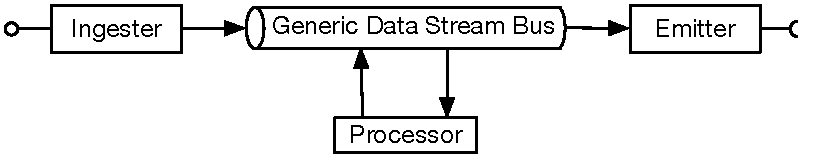
\includegraphics[width=0.9\textwidth]{img/comp-mod-natron-schema}
\caption{Overview of \sti{} architecture.}
\label{fig:sti}
\end{figure} 

Figure~\ref{fig:sti} depicts an overview of the \sti{} internals.
The Ingesters allow ingesting external data flows, and push the data on the Generic Stream Bus. Data items remain in their original format, only the ingestion time is added.
As recommended by the \textit{Lazy Transformation} approach, we postpone the transformation as long as possible in the process. 
The Processors, e.g. an Information Flow Processor as Esper (see Section~\ref{sec:esper-epl}), listens to one or more streams S$\langle\mathrm{T}\rangle$, computes different operations and produces a new stream S$^{\prime}\langle\mathrm{T^{\prime}}\rangle$. 
Emitters allow \sti{} producing a new external data flow in multiple formats. 
In \sti{}, the window operator can be implemented in two different ways: either using the ingestion timestamp added during the Continuous Capturing Phase, or using an application timestamp, e.g. a time mark added during the Augmentation \& Synthesis Phase referring to the notion of Frame in \frappe{}.

\subsection{\protect\sparkdi{} - A Horizontally Scalable Implementation Based on Spark} \label{sec:comp-mod-impl-h-spark}

\sparkdi{} is an implementation of \river{} based on Spark Structured Streaming processing engine (see Section~\ref{sec:spark}). 
It enables the users to create pipeline of streaming computation as they are creating a batch computation, and to leave to the Spark SQL engine to manage the incremental update of the results in a transparent way.

\sparkdi{} offers different implementations of the IN$\langle\mathrm{T}\rangle$ operator that exploits the DataFrames and Datasets API offered by Spark to ingest data from different sources (e.g., filesystem, Kafka, socket, etc.).
In the same way, \sparkdi{} exploits the sink of Spark Structured Streaming as implementations of the OUT$\langle\mathrm{T}\rangle$ operators (e.g., filesystem sink, Kafka sink, Console sink, etc.).
The access to the data, during the Ingestion and Augmentation and Synthesis Phases,  is guaranteed by OBDA techniques implemented in the various components that exploit \frappe{} as data schema.
Moreover, the Dataframe APIs enable the implementation of all the \river{}'s operators and allow the development of the complete stack of layers presented in the \river{} reference architecture (see Section~\ref{sec:comp-mod-sol}).

\begin{figure}[ht]
\begin{minipage}{0.95\linewidth}
\begin{lstlisting}[caption={Example of Window operator in Spark},label=lst:spark-ex,style=SPARKCODE]
   val itemsCounts = inputStream.groupBy(
        window($"ts", "40 seconds", "20 seconds"),
        $"Agg(Count)"
     ).count()
\end{lstlisting}
\end{minipage}
\end{figure}

In particular, the \sparkdi{} implementation of the S2C$\langle\mathrm{T}\rangle$ window operator exploits the native Spark Structured Streaming windowing operations on the ingestion time added to the data during the Continuous Capturing phase.

{Listing~\ref{lst:spark-ex} presents the code to compute the aggregation \textit{Agg(Count)}, representing the amount of the data items that entered the system in the last 40 seconds, using a window that slides every 20 seconds.

\subsection{\protect\hivedi{} - A Horizontally Scalable Implementation Based on Hive} \label{sec:comp-mod-impl-h-hive}
\hivedi{} is a distributed implementation of \river{} computational model based on Hive (see Section~\ref{sec:hive}).
Hive is a Big Data warehouse solution and is not originally ready for managing streaming data.
This limitation can be overcome by chaining, during the Ingestion Phase, the implementations of a IN$\langle\mathrm{T}\rangle$ operator and a S2C$\langle\mathrm{T}\rangle$ operator (window). This chain enable the system to add the ingestion timestamp, \textit{ts} to each incoming data and to transform the time-varying input into a Hive compatible static format (e.g., Parquet) partitioned by \textit{ts}. 
The Augmentation and Synthesis Phase exploits OBDA techniques to access data using \frappe{} ontology as data schema.
The \frappe{} Commons Abstractions layer contains the concepts to enrich and transform data according to the \frappe{} conceptual model (e.g., adding a reference to \frappe{} Frame that groups the data items by time and space).
The final result is then served to the user through implementations of different OUT$\langle\mathrm{T}\rangle$ operators that allow the system to save the data in different format (e.g., filesystem, Kafka, websocket).

As for the \sparkdi{}, we now focus on the S2C$\langle\mathrm{T}\rangle$ window operator in \hivedi{} that exploits the Hive window operator. Differently from Spark, the window operator is not natively supported due to the batch nature of the framework. However, if we augment the data items with a frame ID during the Augmentation and Synthesis Phase, tumbling windows can be implemented grouping by Frame ID. 

\begin{figure}[ht]
\centering
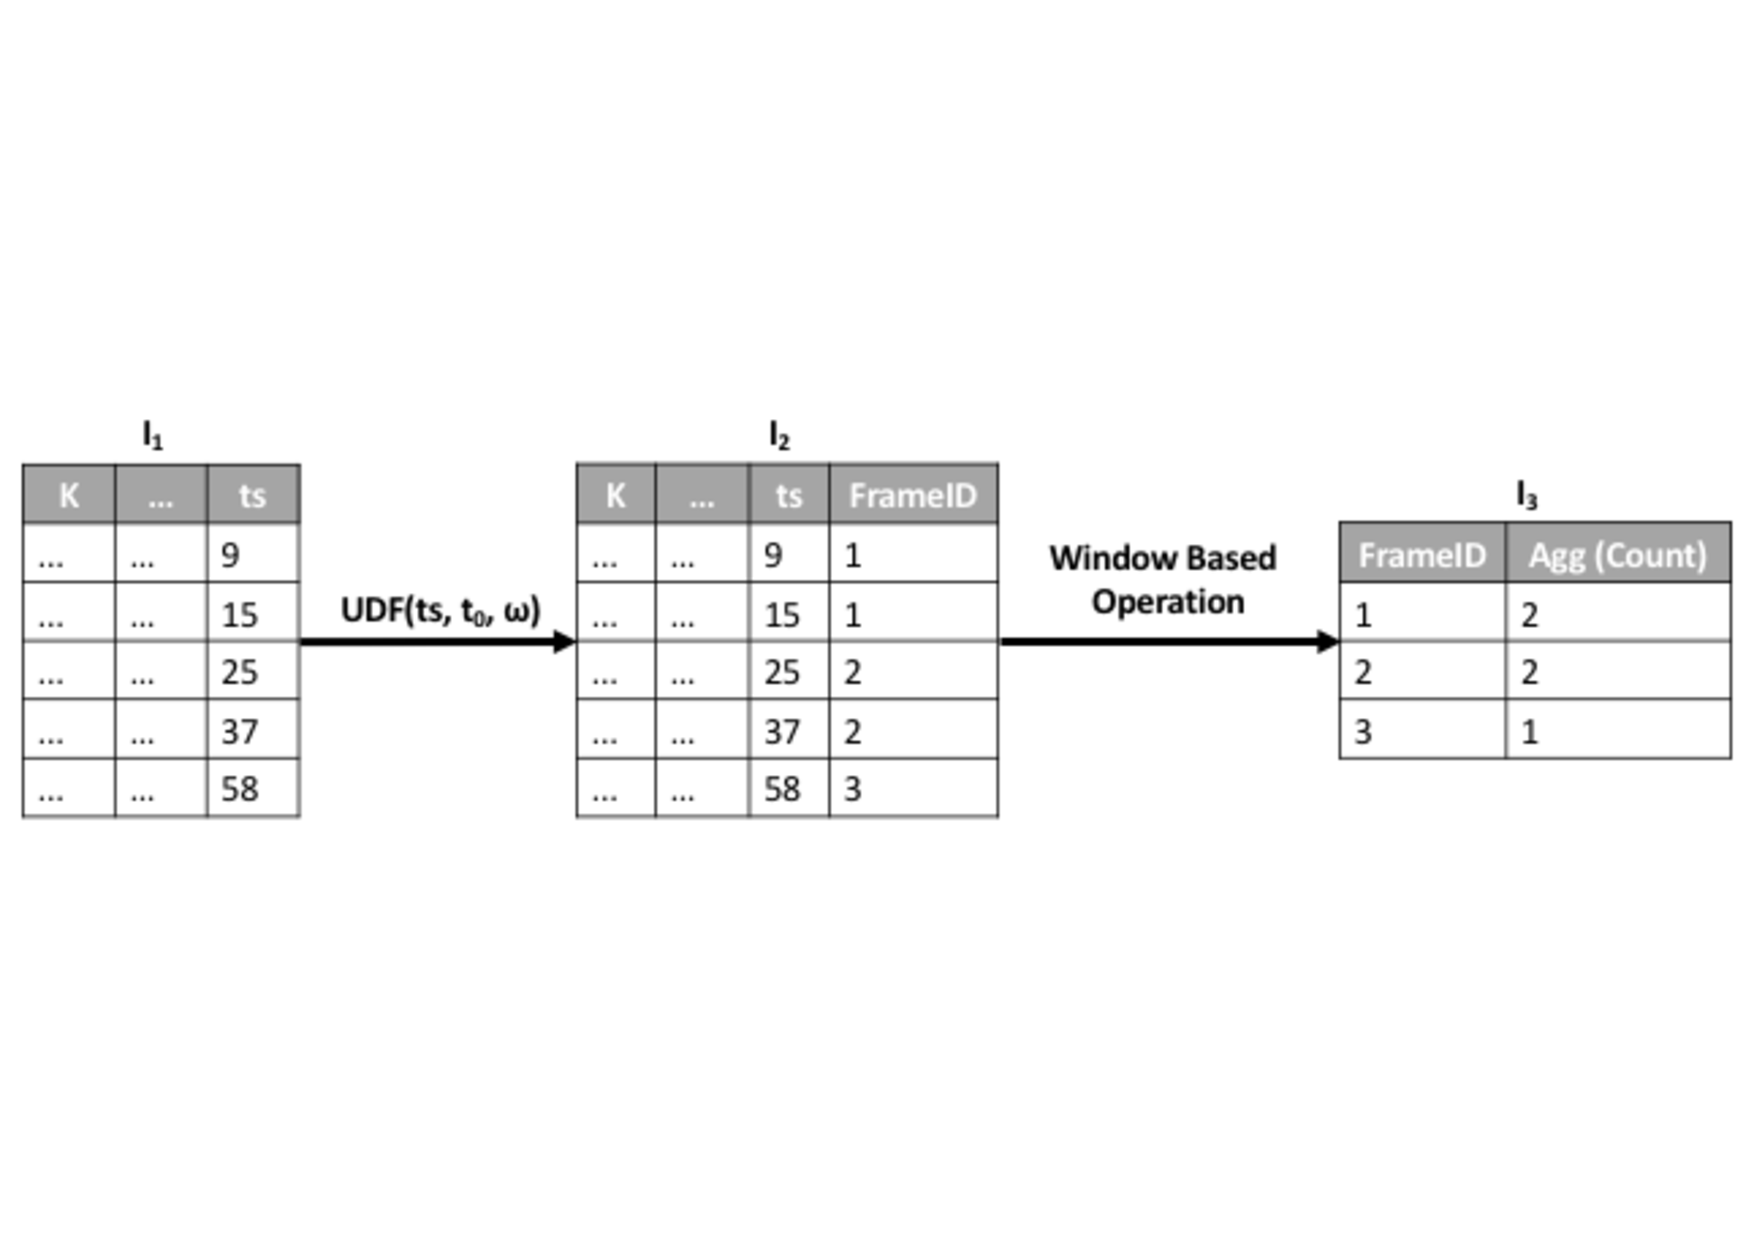
\includegraphics[width=0.92\textwidth]{img/hive_example}
\caption{Example of data operation using hive}
\label{fig:hive-ex}
\end{figure} 

Figure~\ref{fig:hive-ex} shows a simple example of a chain of operations that ingest a data stream, augment it with a Frame ID and simulates a tumbling window that counts the number of data items per frame. \textit{I$_1$} represents the data saved on HDFS during the ingestion phase. \textit{I$_1$} is in form of a table containing various attributes and partitioned by the ingestion timestamp \textit{ts}. The data is augmented using a query that uses a User Defined Function (UDF) to attach a Frame ID based on the \textit{ts} and save the result incrementally in a parquet file partitioned by Frame ID. Such an UDF is configured passing the opening time t$_0$ of the first window, and the length of a Frame  $\omega$. In the example t$_0$ = 0 and $\omega$ = 20. The Frame groups the data items in windows and enables operation on time-varying data in a batch oriented system such as Hive. \textit{I$_2$} represents the augmented data. The Window Based Operation exploits the Frame ID to perform a simple count aggregation by applying a Group by on the Frame ID.  \textit{I$_3$} represents the aggregated data.

\section{Validation of the Lazy Transformation Approach} \label{sec:comp-mod-eval-performace}
%\section{Performance Driven Evaluation: SLD vs. \sti{}} \label{sec:comp-mod-eval-performace}

As a first evaluation step, we compared \sti{} against SLD (see Section~\ref{sec:rsp-mid}). Both of them are single-threaded but, while SLD is based on RDF streams, \sti{} implements the \textit{Lazy Transformation} approach.

Differently from SLD, \sti{} i) uses time-stamped generic data items (instead of focusing only time-stamped RDF graphs) and ii) processes them according to their original nature.
In particular, we test if a system exploiting i) and ii) results a cheaper (using less memory and CPU), faster (reaching higher maximum input throughput) and more accurate (better approximating the correct answer) version of a streaming computational model.

In the following sections, we expose the problem, the solution design and the experimental settings, and, fianlly, we bring experimental evidences that validate the hypothesis \textsf{Hp.2.1}.

\subsection{Problem Settings}
As domain, we chose Social Media analysis as done by the Linked Data Benchmark Council (LDBC) in the SNBench\footnote{\url{http://www.ldbcouncil.org/benchmarks/snb}}. 

SLD and \sti{} receive information in the same way, they both connect to a web socket server and handle JSON-LD files. 

\begin{figure}[ht]
\begin{minipage}{0.95\linewidth}
\begin{lstlisting}[caption={JSON representation of a Twitter micro-post. Due to the lack of space we omitted the context declaration that contains the namespace.},label=lst:json-post, style=JSON]
{"@context": { ... }, 
  "@type": "Collection",
  "totalItems": 1,
  "prov:wasAssociatedWith": "sr:Twitter",
  "items": [{
    "@type": "Post",
    "published": "2016-04-26T15:40:03.054+02:00",
    "actor": {
      "@type": "Account",
      "@id": "user:1",
      "sioc:name": "@streamreasoning"
    },
    "object": {
      "@type": "Content",
      "@id": "post:2",
      "alias": "http://.../2",
      "prov:wasAssociatedWith": "sr:Twitter",
      "sioc:content": "You ARE the #socialmedia!",
      "dct:language": "en",
      "tag": [{
        "@type": "Tag",
        "@id": "tag:3",
        "displayName": "socialmedia"
      }]
    }
  }]
}
\end{lstlisting}
\end{minipage}
\end{figure}

In Listing \ref{lst:json-post}, we propose a JSON-LD serialization of the Activity Stream\footnote{\url{https://www.w3.org/TR/activitystreams-core/}} representation of a tweet as it was injected during the experiments in both systems.  
The JSON-LD representation of an Activity Stream is a \textit{Collection} (specified by \textit{@type} property) composed by one or more social media items. The \textit{Collection} is described by two properties, i.e., \textit{totalItems} and \textit{prov:wasAssociatedWith}, which tell respectively the number of items and the provenance of the items. The collection in the example contains a \textit{Post} created on \textit{2016-04-26} (\textit{published} property) by  an \textit{actor} (Line 6) that produce the \textit{object} (Lines 7-13). 
The \textit{Actor} has a unique identifier  \textit{@id}, a \textit{displayName}, a \textit{sioc:name} and a \textit{alias}. The \textit{Object} has a \textit{sioc:content}, a \textit{dct:language}, zero or more \textit{tag}s, and optionally a \textit{url} and a \textit{to} to represent, respectively, links to web pages and mentions of other actors.

\begin{figure}[ht]
\begin{minipage}{0.95\linewidth}
\begin{lstlisting} [caption={RDF N3 representation of a Twitter micro-post},label=lst:rdf-post, style=N3]
<post:2> a sma:Tweet ;
  dcterms:created "2016-04-26T15:40:03.054+02:00"^^xsd:dateTime ;
  dcterms:language "en"^^xsd:string ;
  sioc:content "You ARE the #socialmedia!"^^xsd:string ;
  sioc:has_container "Twitter"^^xsd:string ;
  sioc:has_creator <user:1> ;
  sioc:id "2"^^xsd:string ;
  sioc:link "http://.../status/2"^^xsd:string ;
  sioc:topic <tag:3> .
<tag:3> a sioct:Tag ;
  rdfs:label "socialmedia"^^xsd:string .
<user:1> a sioc:UserAccount ;
  sioc:account_of "StreamReasoning"^^xsd:string ;
  sioc:creator_of <post:2> ;
  sioc:id "1"^^xsd:string ;
  sioc:name "@streamreasoning"^^xsd:string .
\end{lstlisting}
\end{minipage}
\end{figure}

Listing~\ref{lst:rdf-post} shows the RDF produced by the SLD adapter in transforming the JSON-LD in Listing~\ref{lst:json-post}. The translation exploits well known vocabularies, in particular SIOC\footnote{\url{http://sioc-project.org/}} to represent the online community information, PROV-~O~\cite{w3c-prov-o} to track the provenance of an item and DCTERMS\footnote{\url{http://dublincore.org/documents/dcmi-terms/}} to represents information about the \textit{object}.

\subsection{Solution Design and Experimental Settings} 
A test consists of sending a constant amount of synthetic data using the JSON-LD serialization presented in Listing~\ref{lst:json-post}.
The data is sent in chunks three times per minute (i.e. at the 10$^{th}$, the 30$^{th}$ and the 50$^{th}$ seconds of the minute).  Each chunk contains the same amount of posts. We tested the configuration for different rates: 1500 posts per minute (i.e., three chunks of 500 posts), 3000 posts per minute, 6000 posts per minute, 9000 posts per minute, 12000 posts per minute and 18000 posts per minute.

The rates and the input methodology test a normal situation for SLD (1500 and 3000 posts per minutes) as well as situations that we know to overload SLD (more than 6000 posts per minute)~\cite{DBLP:conf/esws/BalduiniV017a}.

\begin{figure}[t]
\centering
\subfloat[]{
	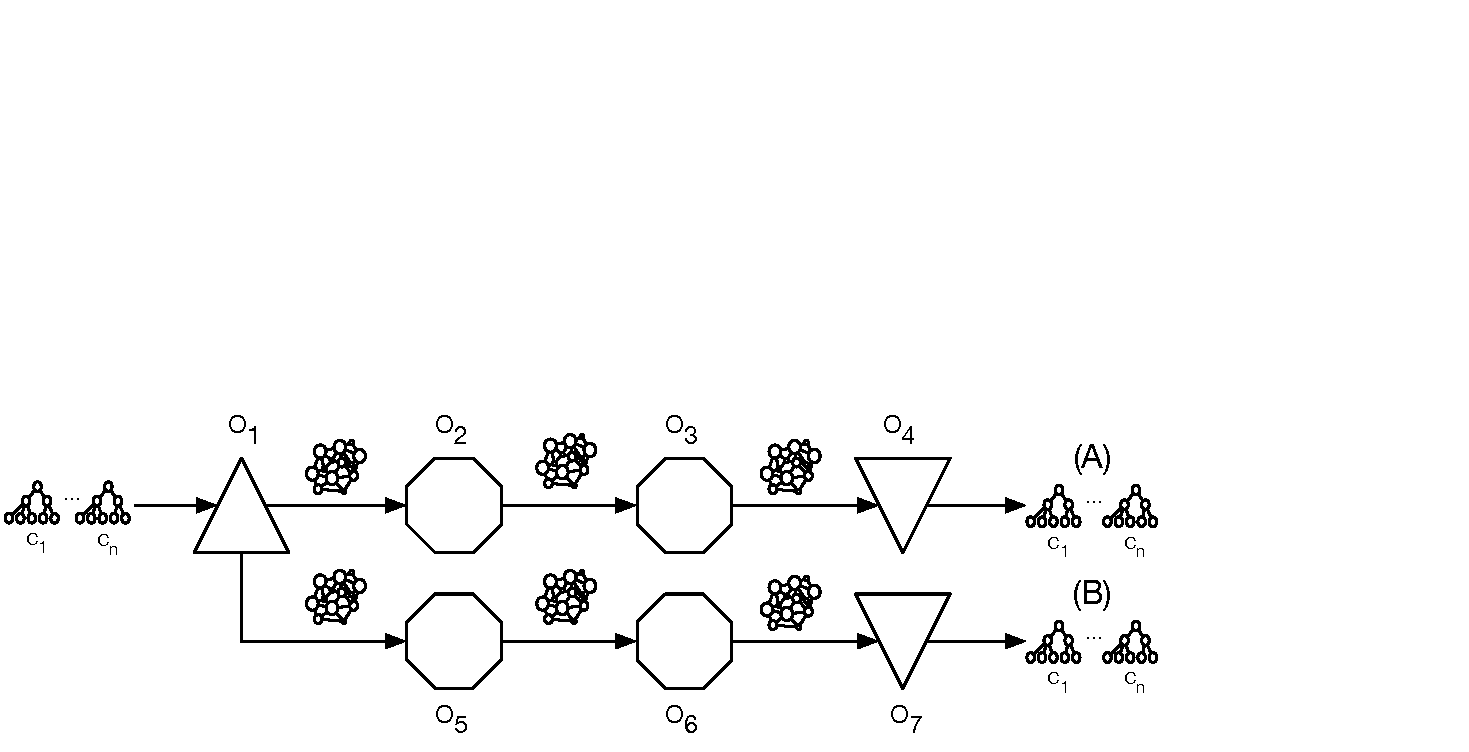
\includegraphics[width=0.8\textwidth]{img/comp-mod-sld-pipeline}
	\label{fig:sld-pl}
} \\
\subfloat[]{
	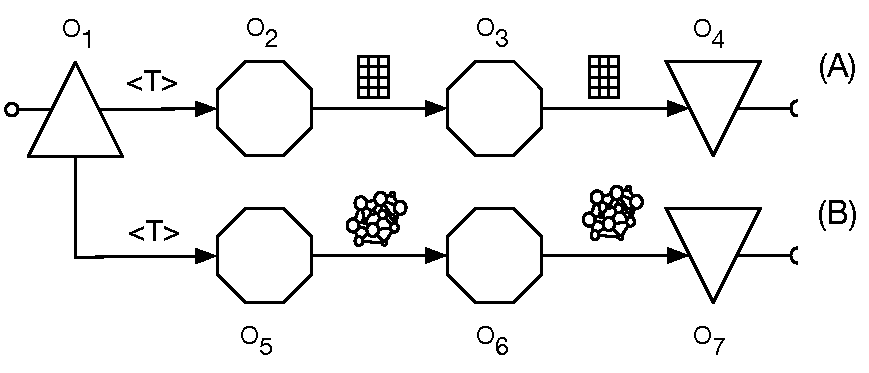
\includegraphics[width=0.8\textwidth]{img/comp-mod-natron-pipeline}
	\label{fig:natron-pl}
}
\caption{(a) SLD pipeline. Even if both the input and the output data are in json format, SLD use RDF graph for the internal computation.
(b) \sti{} pipeline. The input and the output data are both in JSON format, \sti{} try to keep the data in tree format as long as possible during the internal computation.
For graphic syntax legend, please refer to Figure~\ref{fig:sti_ex}.}
\end{figure}

We tested SLD and \sti{} with different pipelines (depicted in Figure~\ref{fig:sld-pl} and in Figure~\ref{fig:natron-pl}): an \textit{area chart} pipeline that computes the number of tweets observed over time, and a \textit{bar chart} pipeline that counts how often hashtags appear in the tweets received in the last 15 minutes.
The two pipelines are coded in SLD and \sti{} in two different ways. 
SLD performs the transformations of JSON-LD in RDF by default, on all the input data, independently from the task to perform. \sti{} keeps the data in its original format as much as possible, i.e., it implements the \textit{Lazy Transformations} approach.
In \sti{}, the results can be continuously computed \textit{i}) using a generic sliding window S2C$\langle Tree \rangle$ operator, which works looking only to the time-stamps of the data items in the generic stream, and \textit{ii}) accessing with C2C$\langle Tree \rangle$ operator implemented as a path expression the \textit{totalItems} property in the JSON-LD file, i.e., the number of items in the collection.

Figure~\ref{fig:sld-pl} presents the two pipelines in SLD with PDL.
The input data are translated in RDF as soon as they enter the pipelines by the \textsf{Ingester} O$_1$, an implementation of an IN$\langle\mathrm{T}\rangle$ operator. The computations for the area chart and for the bar chart (see the part marked with \textbf{A} and \textbf{B} ) are composed by the same type of components and share the new RDF stream translated by O$_1$.
The pipeline \textbf{A} uses two C-SPARQL queries applied to the stream by the operators O$_2$ and O$_3$. Both of them represent a chain of 3 different \river{} operators (a S2C$\langle\mathrm{T}\rangle$, a C2C$\langle\mathrm{T},\mathrm{T}'\rangle$ and a C2S$\langle\mathrm{T}'\rangle$). 
O$_2$ (see Listing~\ref{lst:csparql-prequery}) applies a tumbling window of 1 minute, while O$_3$ aggregates the results using a 15 minutes time window that slides every minute (see Listing~\ref{lst:csparql-query}). 

\begin{figure}[ht]
\begin{minipage}{0.95\linewidth}
\begin{lstlisting} [caption={C-SPARQL query applied by O$_2$ that count the number of post in the stream from O$_1$ using a tumbling window of 1 minute.},label=lst:csparql-prequery, style=CSPARQL]
REGISTER STREAM presocialstr AS 
CONSTRUCT { ?id sma:twitterCount ?twitterC } 
FROM STREAM <http://.../socialstr> [RANGE 1m STEP 1m] 
WHERE { 
    SELECT (uuid() AS ?id) ?twitterC 
    WHERE { 
        SELECT (COUNT (DISTINCT ?mp) AS ?twitterC) 
        WHERE { ?mp a sma:Tweet } 
    } 
}
\end{lstlisting}
\end{minipage}
\end{figure}

\begin{figure}[ht]
\begin{minipage}{0.95\linewidth}
\begin{lstlisting} [caption={C-SPARQL query applied by O$_3$ that aggregates the results from O$_2$ using a 15 minutes time window that slides every minute.},label=lst:csparql-query, style=CSPARQL]
REGISTER STREAM ac AS 
CONSTRUCT { ?uid sma:twitterCount ?totTwitter ; 
              sma:created_during ?unixTimeFrame 
          } 
FROM STREAM <http://.../presocialstr> [RANGE 15m STEP 1m] 
WHERE { 
  SELECT (uuid() AS ?uid) 
         ?unixTimeFrame 
         (SUM(?twitter) AS ?totTwitter)
  WHERE { ?id sma:twitterCount ?twitter ; 
            sma:created_during ?timeFrame . 
          ?timeFrame a sma:15mTimeFrame ; 
            sma:inUnixTime ?unixTimeFrame  
        } 
  GROUP BY ?unixTimeFrame 
}
\end{lstlisting}
\end{minipage}
\end{figure}

It is worth to note that the first query is an important optimization in terms of memory consumption. It avoids the engine to keep 15 minutes of tweets only to count them. In SLD, we often use this design pattern, we call this first query a \textit{pre-query}.
Pipeline \textbf{B} also exploits this design; it applies a pre-query through the O$_5$ operator to reduce the amount of data and, then, a query to produce the final result through the O$_6$ operator. 
It is also worth to note that all the C-SPARQL queries use the form REGISTER STREAM ... AS CONSTRUCT ..., because RDF streams are the only means of communication between SLD components.
The OUT$\langle\mathrm{T}\rangle$ operators of both pipelines, namely O$_4$ and O$_7$, make the results available to processes outside SLD. In this case, both O$_4$ and O$_7$, write JSON files on disk.

Figure~\ref{fig:natron-pl} presents the pipelines in \sti{}. As for SLD, the pipeline \textbf{A} is for the area chart, while \textbf{B} is for the bar chart. 
Differently from the \textsf{Ingester} in the SLD pipeline, O$_1$ does not apply any transformation to the input stream, and the data flows in \sti{} in JSON-LD format.
The O$_1$ operator applies a generic EPL query (presented in Listing~\ref{lst:epl-query}) characterized by a 1 minute long time window.
The clauses \texttt{FORCE\_UPDATE}\footnote{The FORCE\_UPDATE flow control keyword instructs the view to post an empty result set to listeners if there is no data to post for an interval. Note that FORCE\_UPDATE is for use with listeners to the same statement and not for use with named windows. Consider output rate limiting instead.} and \texttt{START\_EAGER}\footnote{The START\_EAGER flow control keyword instructs the view to post empty result sets even before the first event arrives, starting a time interval at statement creation time. As when using FORCE\_UPDATE, the view also posts an empty result set to listeners if there is no data to post for an interval, however it starts doing so at time of statement creation rather then at the time of arrival of the first event.} tell the stream processing engine, respectively, to emit also empty reports and to start processing the window as soon as the query is registered (i.e., without waiting for the first time-stamped data item to arrive).
It is worth to note that this query exploits the event-based nature of the generic stream it is observing.
It does not inspect the payload of the events; it only uses their time-stamps.

\begin{figure}[ht]
\begin{minipage}{0.95\linewidth}
\begin{lstlisting} [caption={The generic window query applied by the operator O$_1$.},label=lst:epl-query,numbers=none, style=ESPER]
SELECT * 
FROM event#TIME(1 min,"FORCE_UPDATE, START_EAGER")
\end{lstlisting}
\end{minipage}
\end{figure}

As explained in Section~\ref{sec:comp-mod-impl-v}, processors are the central components of \sti{}. They can listen to one or more generic stream, compute different operations and push out a generic streams. The type of the input and output streams can be different. The two pipelines use different processors (e.g. RDF translator, windower and SPARQL).

\sti{} maintains the data format as long as possible in order to reduce the overhead of the translations. It can exploit the tree-based nature of JSON-LD. In pipeline \textbf{A}, the operator O$_3$ exploits a path expression data to extract \textit{totalItems}, i.e., the number of items in each collection, from the time-stamped JSON-LD items in the generic stream it listens to. It outputs a tuple $\langle$timeframe,count$\rangle$ that is aggregated every minute over a window of 15 minutes using an EPL statement.

The pipeline \textbf{B} of \sti{} shares the O$_1$ operator with the pipeline \textbf{A}.
The operator O$_5$ translates the generics in input in RDF graph. This transformation is required to extract information about the hashtags. As for the pipeline \textbf{B} of SLD, we use a pre-query design pattern to reduce the amount of data. A SPARQL processor, implementing the operator O$_5$, applies the SELECT query in Listing~\ref{lst:sparql-prequery} to every data-item in the stream and pushes out a stream of tuples $\langle$hashtagLabel,count$\rangle$. The relational stream is then aggregated with an ESPER processor, which implements O$_6$, with a 15 minute time window that slides every 1 minute (see Listing~\ref{lst:epl-query-bc}). 

\begin{figure}[ht]
\begin{minipage}{0.95\linewidth}
\centering
\begin{lstlisting} [caption={SPARQL pre-query applied by the component O$_6$},label=lst:sparql-prequery, style=SPARQL]
SELECT ?htlabel (COUNT(DISTINCT(?mpTweet)) AS ?htTweetCount) 
WHERE { ?mpTweet a sma:Tweet ; sioc:topic ?tweetTopic . 
        ?tweetTopic a sioctypes:Tag ; rdfs:label ?htlabel } 
GROUP BY ?htlabel 
ORDER BY DESC(?htTweetCount) 
\end{lstlisting}
\end{minipage}
\end{figure}

\begin{figure}[ht]
\begin{minipage}{0.95\linewidth}
\begin{lstlisting} [caption={EPL query for the bar chart, applied to the stream by the component O$_6$},label=lst:epl-query-bc,numbers=none, style=ESPER]
SELECT htlabel, SUM(count) as sumHt 
FROM HTCountEvent#TIME(15 min) 
GROUP BY htlabel 
OUTPUT SNAPSHOT EVERY 1 min 
\end{lstlisting}
\end{minipage}
\end{figure}

As for SLD pipelines, the operators O$_4$ and O$_7$ of the \sti{} pipelines are implementations of \textsf{Emitter}s and offer the result to the user in the form of JSON files on disk.

\subsection{Results and Discussion}\label{sec:comp-mod-eval-performace-res}
As key performance indicators (KPIs), we measure  the resources consumption of the two systems and the correctness of the results. For the resource consumption, we measure every 10 seconds: \textit{i}) the CPU load of the system thread in percentage, \textit{ii}) the memory consumption of the thread in MB and \textit{iii}) the memory consumption of the Java Virtual Machine (JVM). For the correctness, we compared the computed results with the expected results. Being the input a constant flows of tweets that only differ for the ID, the area chart is expected to be flat and the bar chart is expected to count exactly the same number of hashtags every minute.

\begin{figure}[t]
\centering
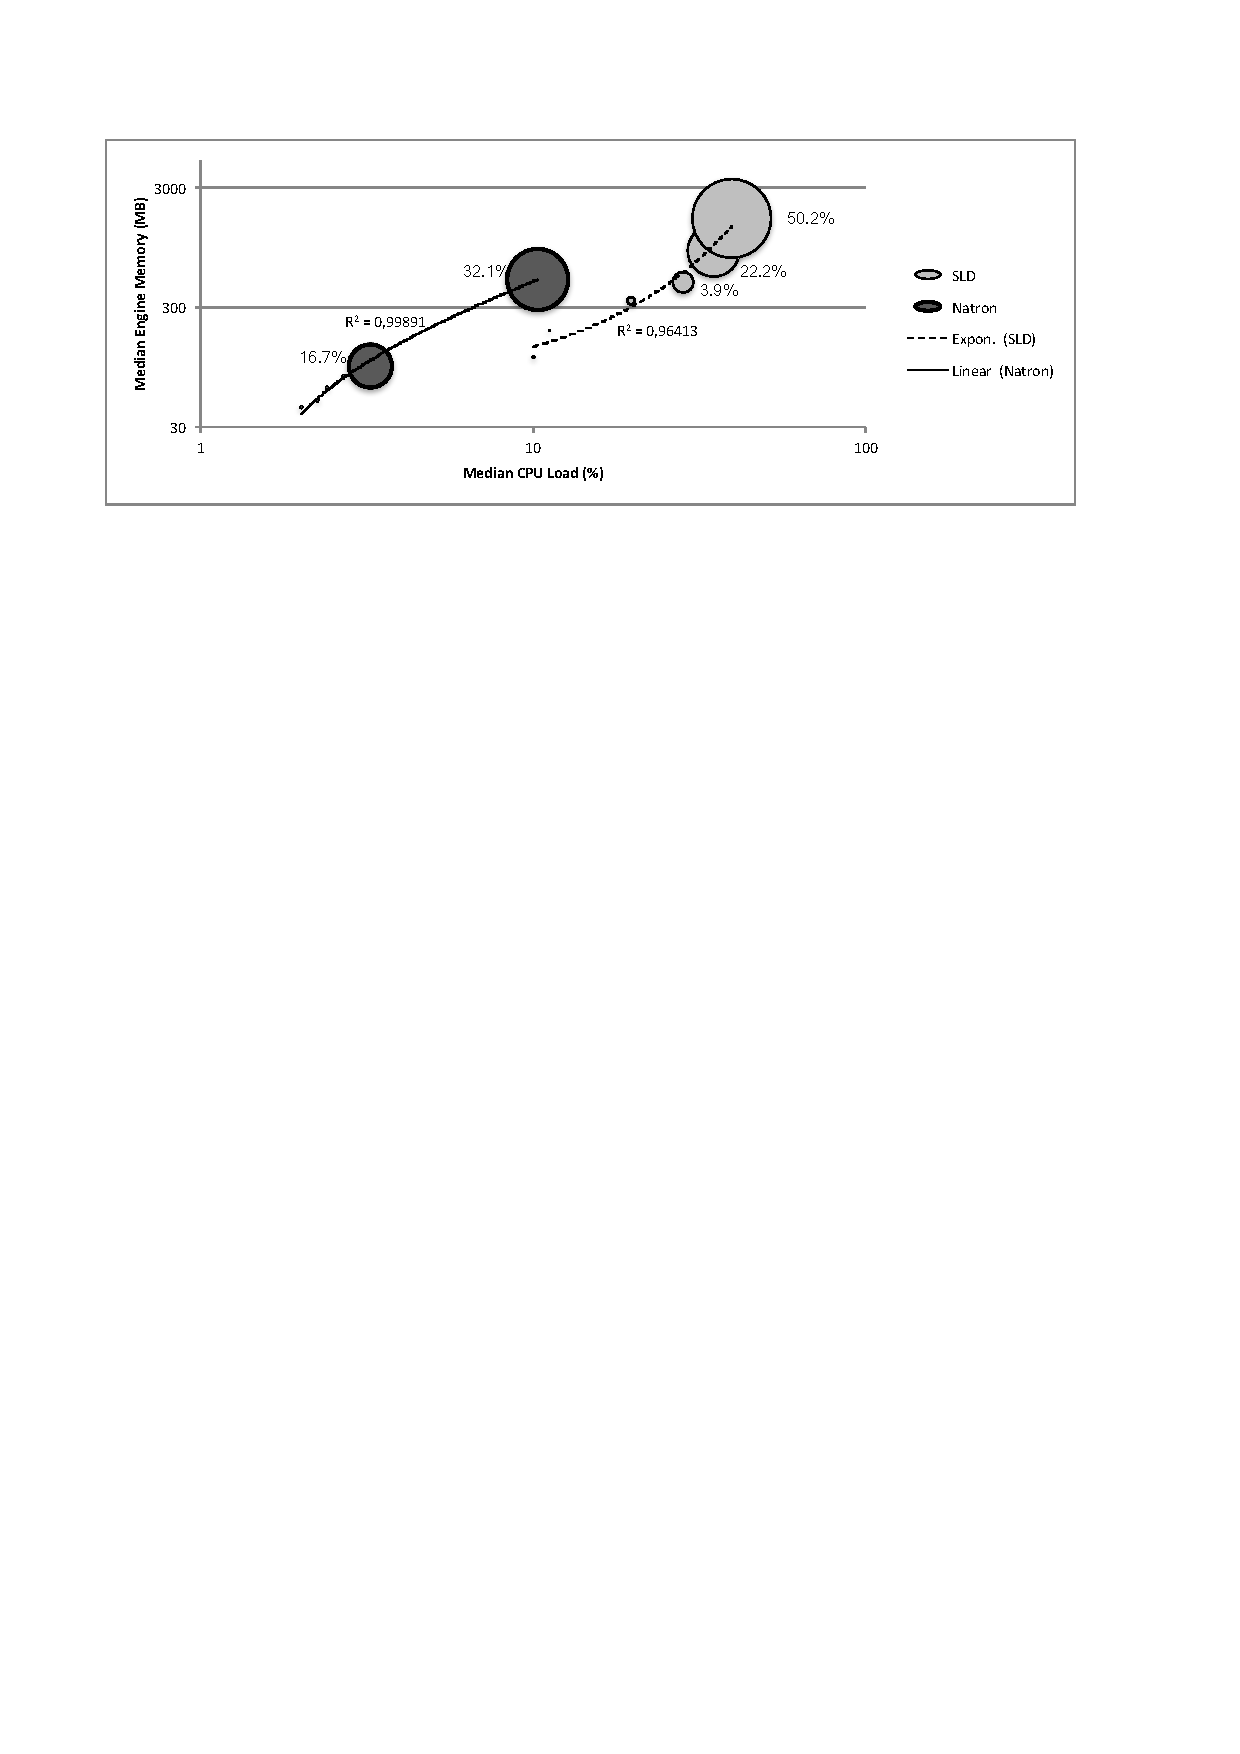
\includegraphics[width=\textwidth]{img/comp-mod-cpu-mem-acerror}
\caption{An overview of the experimental results; larger  bubbles means greater \% errors.}
\label{fig:cpu-mem}
\end{figure}

\begin{figure}[t]
\centering
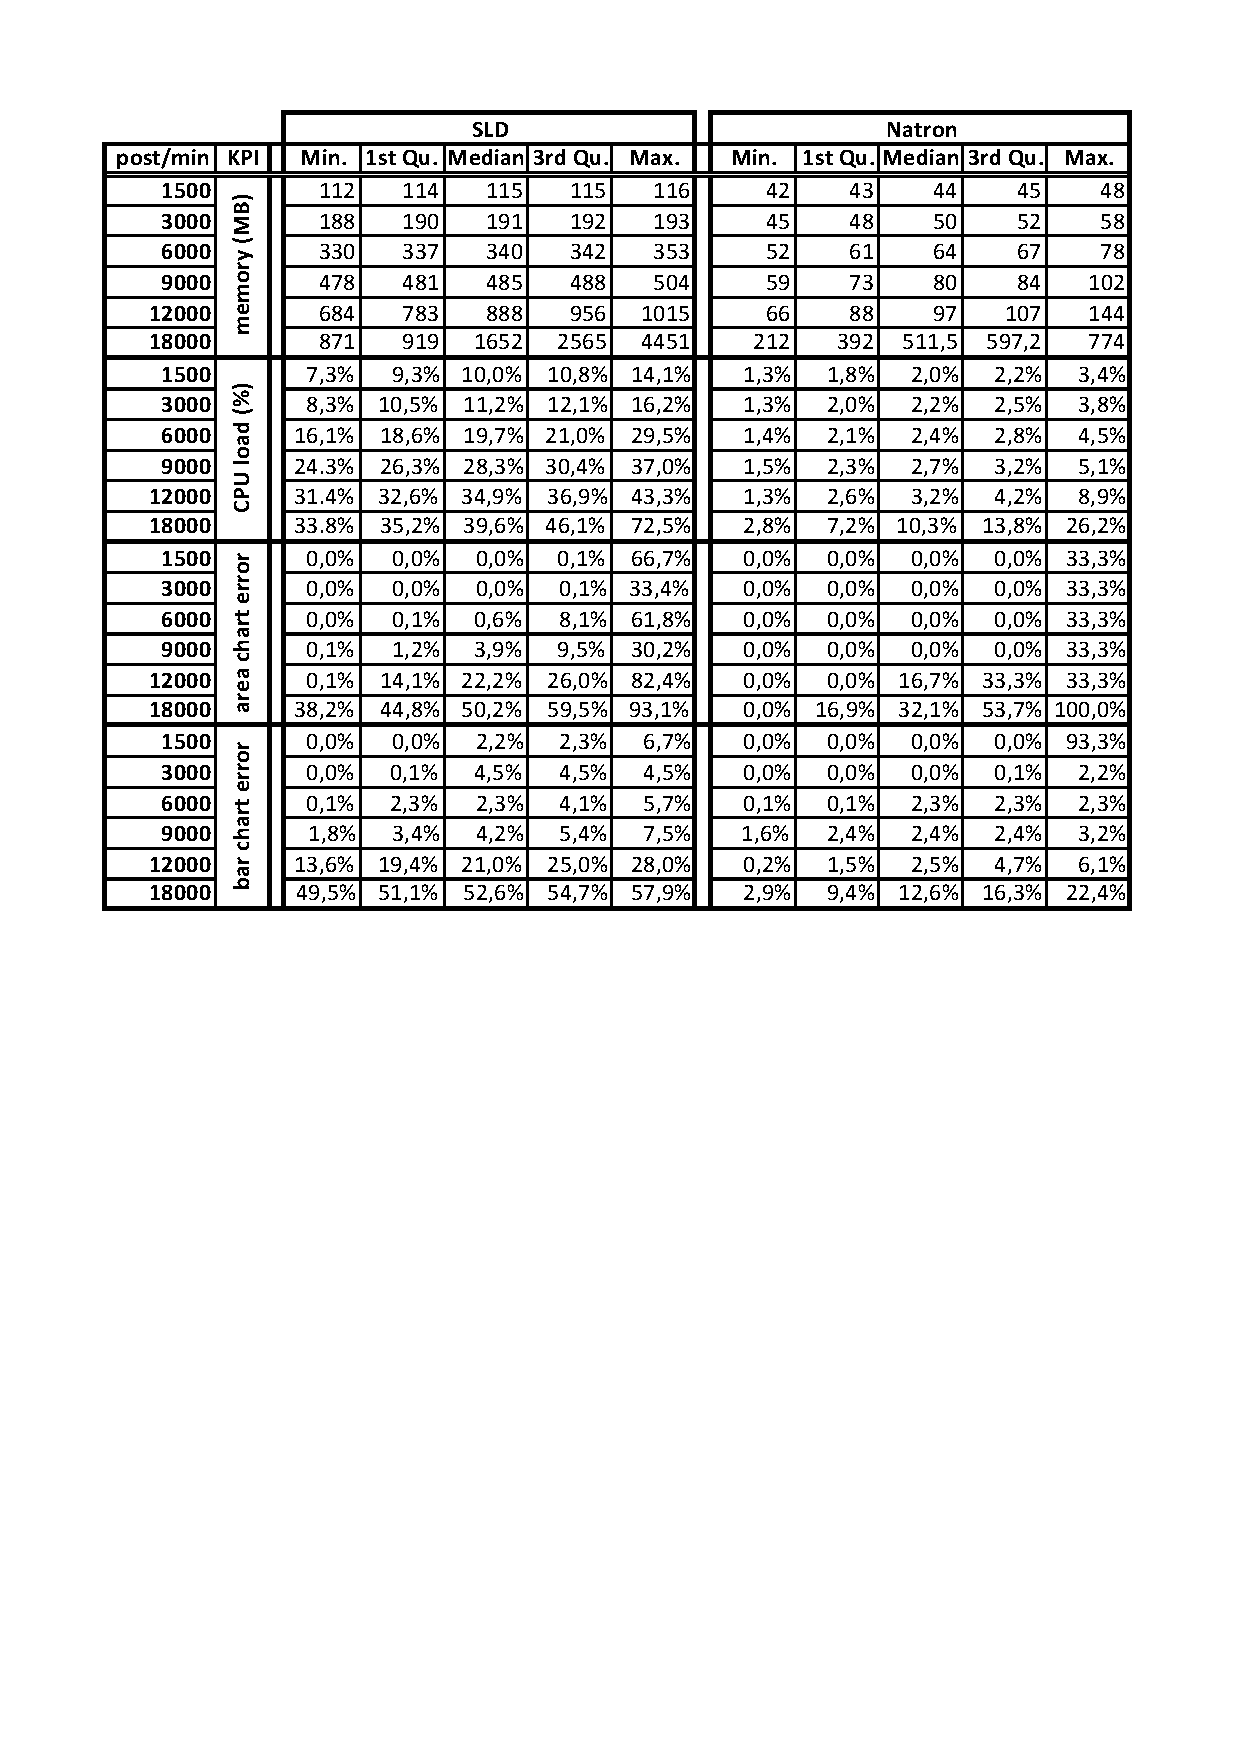
\includegraphics[width=\textwidth]{img/comp-mod-results}
\caption{The experimental results.}
%\vspace{-0.5cm}
\label{fig:all-data}
\end{figure}

Figure~\ref{fig:cpu-mem} offers an overview of the results of the experiments. The full results are reported at the end of this section in Figure~\ref{fig:all-data}. On the X, axis we plot the median of the CPU load in percent, while on the Y axis, we plot the memory allocated by the engine thread. The size of the bubble maps the median of the error of the area chart. Bubbles in the lower left corner correspond to the experiment where we sent 1500 tweets per minute.

Increasing the throughput results in more memory consumption and CPU load for both systems. However, \sti{} consumes less memory than SLD and occupies less CPU. Moreover, \sti{} presents a linear increment for both these KPIs, while the resource usage for SLD grows exponentially with the throughput (note the R$^2$ in Figure~\ref{fig:cpu-mem}). Also the error in the results increases with the throughput: SLD already shows an median error greater than 3\% in the bar chart at 3000 tweets per minutes and in the area chart at 9000 tweets per minute; \sti{} is faster - i.e. it reaches higher maximum input throughput - and more accurate -- i.e. it reaches 3\% error level only for 18000 tweets per minutes, providing more precise results than SLD.

Figure~\ref{fig:timeplots} presents the recorded time-series for CPU load and memory usage in both systems. The memory usage graphs contain two different time series. The blue one represents the memory usage of the system thread, while the orange one shows the total memory usage for the JVM.

\begin{figure}[p]
\centering
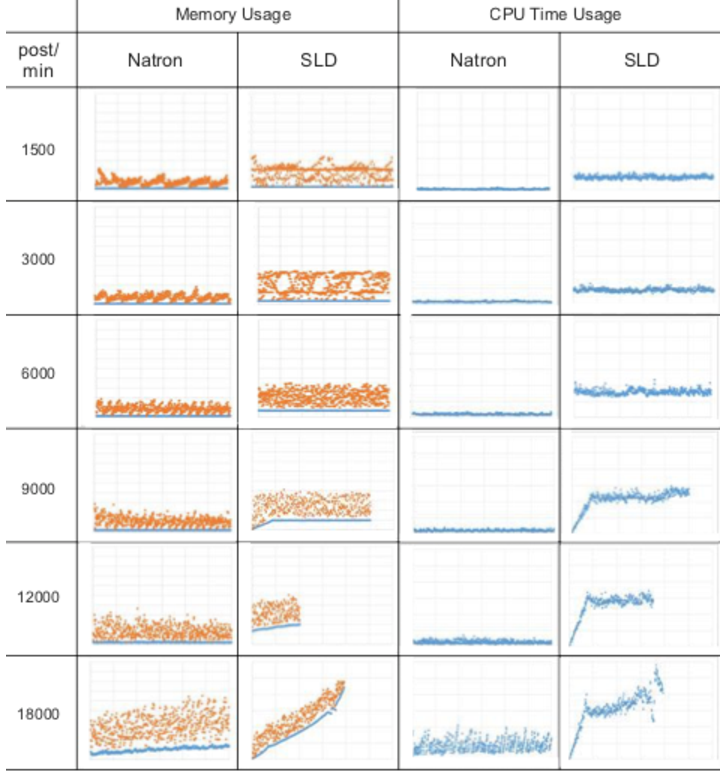
\includegraphics[width=\textwidth]{img/comp-mod-timeplots}
\caption{Memory and CPU usage over time. In the Memory Usage columns, the blue dots represents the memory usage of the system thread, while the orange dots shows the total memory usage for the JVM. In the CPU Time Usage columns, the blue dots represents the CPU time usage of the system thread.}
\label{fig:timeplots}
\end{figure}

The memory usage of the system thread accounts for all the components and data in the pipeline. Notably, when the system under testing is not overloaded, the memory usage is constant over time, while when the system is overloaded it grows until the system crashes. The total memory usage of the JVM shows, instead, the typical pattern of the garbage collector that lets the JVM memory grow before freeing it. Also in this case, when the system it is overloaded, the garbage collector fails to free the memory.

During the experiments the median of the  memory used by SLD spans from 115 MB, when loaded with at 1500 posts/min, to 1.6 GB, when loaded with 18000 posts/min. For \sti{}, instead, it spans from 44 MB to 511.5 MB in the same load conditions. The experimental results clearly shows that \sti{} consumes (in average) three times less memory than SLD.

\begin{figure}[p]
\centering
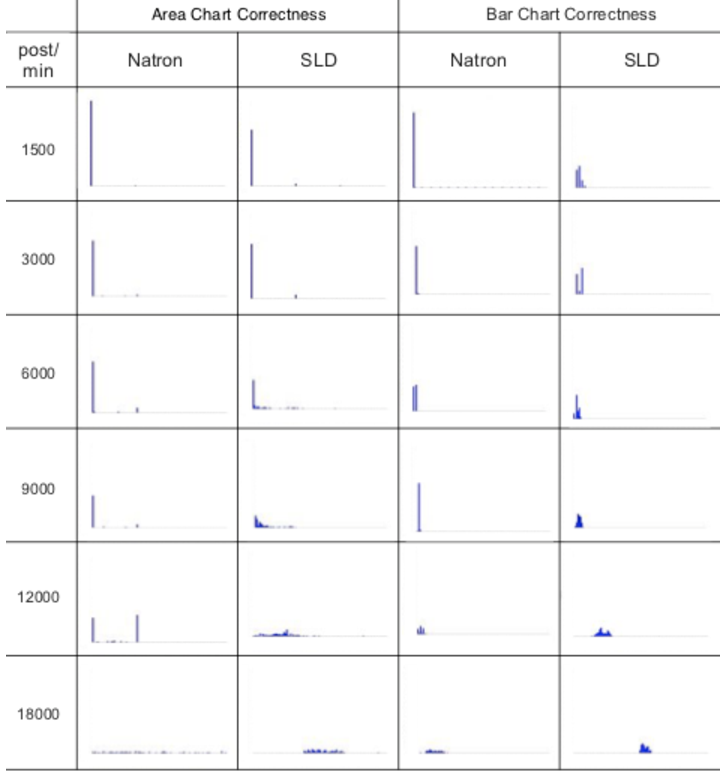
\includegraphics[width=\textwidth]{img/comp-mod-errors}
\caption{Area chart and bar chart errors distributions}
\label{fig:errors}
\end{figure}

The same considerations can be proposed for the CPU load. The median of the CPU load spans  from 2\% to 10\% for \sti{}, while it spans from 10\% to 39.5\% for SLD. \sti{} consumes in average 4 time less CPU time than SLD. 
Moreover, it offers higher level of stability for both the parameters in all the experiments. 

The correctness results are summarized in Figure~\ref{fig:errors}. The X axis of each plot shows the percentage of error; it ranges from 0\% to 100\%. The Y axis is the percentage of results with that error; it also ranges from 0\% to 100\%. A bar as tall as the Y axis in the left side of the graph means that all results where correct. The smaller that bar is and the greater the number of bars to the right is, the more errors were observed.

In general, the results show that \sti{} is more accurate (the result error is smaller) than SLD and, consequently, validate the hypothesis \textsf{Hp.2.1}. For the area chart the distribution shows that \sti{} percentage of error is very low when the input throughput is between 1500 posts/min and 9000 posts/min. When it is higher (i.e., 12000 and  18000 posts/min) also \sti{} starts suffering and the percentage of errors starts growing. For SLD, errors are present even at lower input rate, the graph shows that the error distribution starts moving to the right at 6000 posts/min. Similar consideration can be proposed for the bar chart error distribution. The degradation of performance of SLD starts a very low rate, a substantial presence of errors around 7\% can be seen with 6000 posts/min in input.

Figure~\ref{fig:timeplots} and Figure~\ref{fig:errors} show the deep correlation between resources usage and errors. Clearly, a growing input throughput drives the systems to be less reliable. For both \sti{} and SLD the correctness of the results decreases as soon as the machine is overloaded and the resources usage starts rising out of control.

{\color{red}
Differently from SLD, that uses only the ingestion time to optimize the reactiveness, \sti{}, also accept the application time. It guarantees the accuracy of the computation at the expense of reactiveness. 
It is worth to note that it is important to find a good trade-off between the two KPIs, this trade-off is domain dependent. 
}

\section{COST-Aware Evaluation: Distributed vs. Single-Threaded} \label{sec:comp-mod-eval-cost}
%\section{COST Driven Evaluation} \label{sec:comp-mod-eval-cost}
In~\cite{DBLP:conf/debs/BalduiniPV18}, in order to validate the hypothesis \textsf{Hp.2.2} and inspired by COST (see Section~\ref{sec:bench-cost}), we propose an empirical comparison between a \sparkdi{} and \sti{} for a streaming data analysis task. The focus of our analysis is less on performance, and more on the total cost of solving the task. This shift is motivated by the industrial setting in which this work is conceived. In industry, solutions must be evaluated both in terms of cost-effectiveness and efficacy. The research question we want to answer is -- \textit{What is the most cost-effective solution for streaming data analysis when comparing distributed and single-threaded deployments?}

It is well established that performance metrics are frail when they ignore cost-related indexes (see Section~\ref{sec:dsb}). For this reason, differently from previous works~\cite{arasu2004linear,chintapalli2016benchmarking} that focuses on latency and throughput, we base our analysis on the total solution cost. This cost is obtained by multiplying the price-per-second of the machines storing the data and running the solution by the execution time needed for the analysis task. With this choice, we want to highlight the cost-effectiveness of a solution.

Our use case is an on-line anomaly detection task. Our goal is to detect unusually crowded areas in a city. Our dataset consists of the mobile phone connection data collected in Milan during 2016 (see Section~\ref{sec:cs-mdw-2016}). The possibility to perform this task is well documented in~\cite{krings2009urban,calabrese2010geography,calabrese2011real}. Both of our solutions use the same anomaly detection strategy. This consists in a statistical model-based anomaly detector trained on historical data~\cite{DBLP:journals/ieeemm/BalduiniVALAC15} (for more information, see Chapter~\ref{ch:case-studies}). 

We compare the performance of \sparkdi{} and \sti{}.
In both cases, RDF is not used at all and data are kept in their format as long as possible.
In the follows, we describe the tuning of both solutions to our particular use case. Then, we compare them on the total cost required to solve the anomaly detection task. In order to assess the solutions' scalability, the analysis is replicated multiple times and for different data volumes.

The design of an industrial solution also requires operational considerations. With the term operational, we refer to the choices regarding when and how data is ingested, stored, and processed. Depending on the use case, there might be different operational requirements. In our use case, data is generated continuously from the mobile phone network. To avoid data losses, our only operational requirement is that data must be ingested continuously (see Section~\ref{sec:comp-mod-intro}). For our analysis, we consider the following two consumption policies: (i) \textit{continuous} -- data is consumed in real-time as soon as it is ingested -- and (ii) \textit{periodic} -- data is consumed at regular time intervals (e.g., once a day, or  once a week). Those choices influence the total solution cost. For example, if we want to analyze data continuously, we need dedicated hardware running 24/7.

\subsection{Problem Settings}\label{sec:comp-mod-eval-cost-prob}
%\subsubsection{Data Description}
\label{sec:desc}
% Mobile phone data can offer relevant and real-time hints about the presence of people in a geographical area~\cite{balduini2015citysensing,DBLP:journals/pervasive/CalabreseKRBFBKFWMFGBNPTBKHSSMK07,calabrese2011real,krings2009urban,calabrese2010geography,della2015listening}. 
% Such analyses can be used to describe a territory's macro-dynamics. In particular, we refer to mobile phone connection data, commonly known as \textit{Call Detail Records} (or CDRs). Every mobile phone generates a CDR every time a call, SMS or Internet connection is made. The CDR contains information about the customer, the type of connection, and the cellular tower instantiating the connection. This data is used by telco companies for billing purposes.

% Each CDR can be associated to a base tower, and each tower can be associated to a geographical location. Then, it is possible to map mobile phone activity to geographical locations. The number of active mobile phones at a location, computed following a privacy-preserving methodology, can approximate the number of people in the area. To make analysis more understandable, the mobile network is often approximated with a regular grid\footnote{For an industrial implementation of this solution see TIM Big Data \url{https://www.olivetti.com/en/retail/data-driven-solutions/tim-big-data}}. In our case, each grid cell represents a 250x250 meters square. We term each square a \textit{pixel} and we represent the city as a series of frames composed by pixels \cite{DBLP:conf/semweb/BalduiniV15}.

In this work, we use mobile phone data, in particular the CDRs (see Section~\ref{sec:uda-motivation}), collected in the city of Milan, Italy, during the months of February, March, April and June 2016. Data was made available thanks to the collaboration with TIM -- Telecom Italia.

We model data using \frappe{} (see Chapter~\ref{ch:conceptual}) .
The city was overlaid by a \textsf{Grid}, each grid \textsf{Cell} represents a 250x250 meters square. 
In order to preserve user privacy, data is aggregated at \textsf{Pixel} level using 15-minutes-long \textsf{Frame}s.
Consequently, we created a film of \textsf{Frame}s, which shows the evolution of the city, by counting the number of distinct mobile phone users in each \textsf{Pixel}. For privacy preserving reasons, if the counting goes below a given threshold, it is set to zero.

The data collected in the month of April is the most significant; in this period the city of Milan hosts a design festival\footnote{\url{http://archivio.fuorisalone.it/2016/en}} that attracts half a million of visitors, and an anomalous density of people can be detected in the 11 districts of Milan that host the 1.151 events~\cite{DBLP:journals/ieeemm/BalduiniVALAC15} of the festival. This dataset comprises CDRs of calls and SMSs collected between April 13th and April 17th 2016. CDRs of Internet connections are filtered out since this data is missing in the majority of the months considered. This one-week dataset occupies 1.7GB, and contains around 24 millions calls and 17 millions SMS records. We name this dataset Mobile 1, and we shorten it as MOB1. 

We use the rest of the data (March, February, June) for training the models described in Section \ref{sec:comp-mod-eval-cost-prob}. The cost of this activity is not considered in the paper.

In order to include the scalability dimension in our analysis, we generated several datasets by scaling our original MOB1 dataset. The scaling procedure takes as input an integer scaling factor $k$, and it replicates each CDR in the dataset $k$ times.

Through scaling, we generated several additional datasets for our experiments. The most representative ones are:
\begin{itemize}
\item MOB1 (1.7GB), original dataset, representative of weekly mobile traffic (excluding Internet connections) in a large metropolitan area (Milan).
\item MOB10 (17GB), $k = 10$, representative of weekly mobile traffic (including Internet connections) in a large metropolitan area (Milan).
\item MOB30 (50GB), $k = 30$, representative of weekly mobile traffic in a country (Italy).
\item MOB50 (83GB), MOB100 (170GB), extreme situations.
\end{itemize}
Representative sizes are based on internal TIM metrics. Unfortunately, all datasets used in this study are not available for public disclosure under TIM policies. Aggregated data similar to the one we produced internally when processing the raw CDRs is available as part of the TIM Big Data challenge 2015 dataset\footnote{\url{http://www.telecomitalia.com/tit/en/bigdatachallenge.html}}.

In our use case, we are interested in finding out which areas of a metropolitan city are unusually crowded. The people present in a certain area can be approximated by the number of active mobile phones in the area.

We can cast this use case into an on-line time series anomaly detection problem. Anomaly, or outlier, detection is a data analysis task such as classification or clustering \cite{aggarwal2015outlier}. Anomaly detection consists in identifying the most anomalous data patterns in a data set. An anomalous pattern could be composed of a single or several data elements. Anomaly detection relies on the ability of building a model of normality for a system or phenomenon. The model is then used to detect anomalies by computing the ''distance'' between the model and the anomalous element.

In our case, an anomaly represents an infrequent event in the city, which attracts a large number of people. A model of normality can be built by analyzing mobile phone data in periods where no event occurs. This is usually known as \textit{training} in the machine learning community. Then, the trained model is compared with the collected data to detect anomalies.

We perform an online anomaly detection analysis (see Section~\ref{sec:uda-analysis}). 
For training, we consider a the evolution of each \textsf{Pixel}. 
Following \cite{DBLP:journals/ieeemm/BalduiniVALAC15}, we assume each \textsf{Pixel} follows a Gaussian distribution, and we approximate its parameters by computing the sample mean and variance in periods where no sizable event happens (i.e., in February, March, and June). We repeat this process for weekdays and weekends, since they present different mobile activity patterns. This accounts for $2 \times 24 \times 4 = 192$ models for each pixel, i.e., 1.92 million models considering the 10.000 pixels the city is divided in. Anomalies are detected at runtime by joining each pixel measurement with the corresponding model distribution. Measurement $x$ is reported as an anomaly if its z-score is larger than $3$, that is 
\begin{equation}
\label{eq:zscore}
  \frac{|\bar{\mu} - x|}{\bar{\sigma}} > 3
\end{equation}
where $\bar{\mu}$ and $\bar{\sigma}$ are the estimated mean and standard deviation for $x$'s pixel in the corresponding fifteen minutes slot.

Note that there exists a plethora of more advanced anomaly detection techniques (for an extensive reference see~\cite{aggarwal2015outlier}). Finding the most accurate detector is outside the scope of this work. We use the Gaussian model since it has been shown~\cite{DBLP:journals/ieeemm/BalduiniVALAC15} to be well-fit for the problem at hand. In particular, our method can be executed in parallel on a cluster of computers, since every pixel can be analyzed independently from the others. As already mentioned. the only operational requirement for our use case is that data is collected in real-time to avoid data losses.

\subsection{Solution Design} \label{sec:solutions}
The cost of an analytics solution depends on infrastructural, architectural, and operational choices. The proposed solution is a specialization of the reference architecture presented in Section~\ref{sec:comp-mod-sol-arch}.

\begin{figure}[ht]
  \centering
  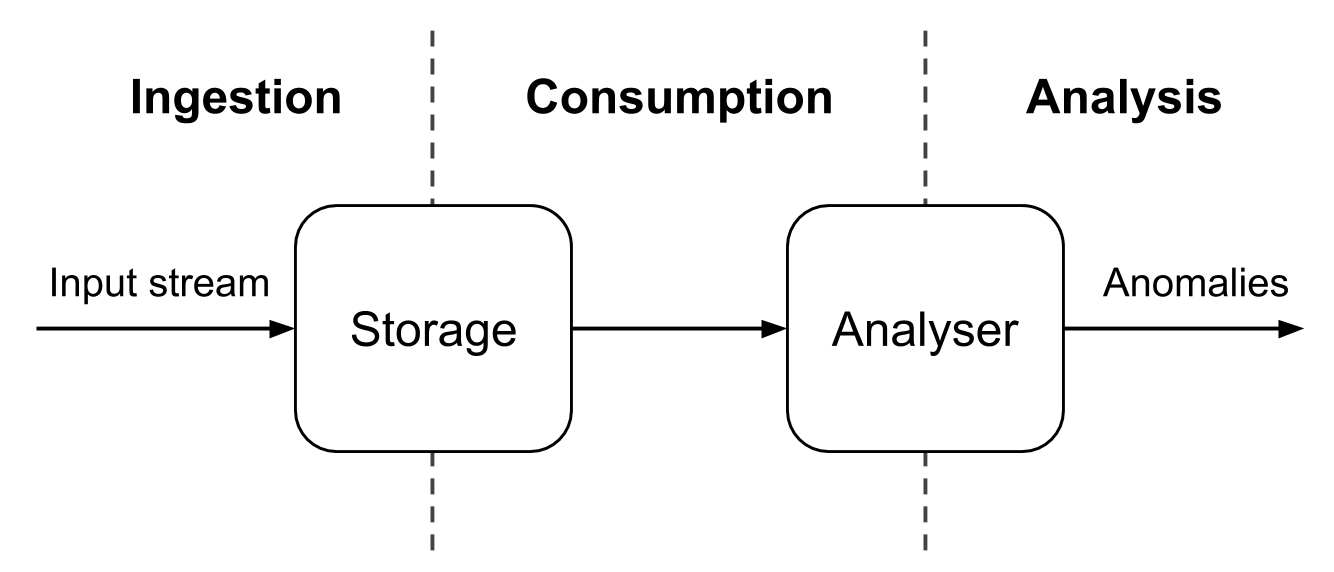
\includegraphics[width=.7\textwidth]{img/eval-arch-1}.
    \caption{General architecture of our solution}
    \label{fig:arch_abs}
\end{figure}

being a specialization of \river{} reference architecture, our data analysis task can be decomposed into three main phases (see Figure \ref{fig:arch_abs}):
\begin{itemize}
\item data ingestion -- data is collected from the mobile network and transferred to a storage layer.
\item data consumption -- data is transferred from the storage layer to the analysis layer.
\item data analysis -- data is processed and results are generated by joining streaming data with the static models.
\end{itemize}

Note that we add a storage layer between ingestion and consumption to decouple the two phases. This means that we can ingest data in real-time, and analyze it at a later stage. This also enables various operational scenarios.
%%
%\paragraph{Infrastructure}
An infrastructural choice specifies where a solution is deployed. The hardware used to run an application can be bought, or rented from a cloud service provider. We restrict our analysis to cloud services, since they usually reduce the operational cost of the solution.

When instantiating virtual machines (VMs), cloud service providers usually offer two types of billing policies: pay-per-use instances and reserved instances. Reserved instances (RIs) can be held for a fixed amount of time at a reduced price with respect to pay-per-use instances. RIs are well-fit to reduce the cost of continuous data analysis solutions, while pay-per-user instances are better fit for bursty workloads, such as periodic analysis tasks. In the following, we refer to pay-per-use instances as shared.

\begin{table}[ht]
  \centering
    \caption{Azure VM sizes (January 2018)}
  \begin{tabular}{@{}lrrr@{}} \toprule
  VM Type & Cores & RAM (GB) & S/R (\euro/month)\\
    \midrule
  VM1 & 2 & 4 & 64.62/60.33\\
  VM2 & 4 & 8 & 127.99/121.58\\
  VM3 & 8 & 16 & 256.61/242.42\\
  VM4 & 16 & 32 & 513.23/484.92\\
    \bottomrule
  \end{tabular}
    \label{tab:sizes}
\end{table}

Table \ref{tab:sizes} presents the characteristics of the virtual machines used in this study. The last column contains the approximated cost of running a shared instance versus a reserved instance. 
The reported costs and characteristics refer to Fsv2-series VMs of Microsoft Azure\footnote{https://docs.microsoft.com/en-us/azure/virtual-machines/windows/sizes-compute}. We chose the Fsv2-series because it is equipped with computation optimized hardware that fitted our needs at affordable cost.
Nevertheless, reported costs do not differ significantly from those of other cloud service providers. 

%\paragraph{Architecture}
%We designed our solutions according to the general architecture depicted in Figure~\ref{fig:arch_abs}. 
%
%The storage layer is responsible for ingesting data in real-time from the mobile network. Due to the arbitrary velocity of the mobile data stream, the streaming storage must be able to scale seamlessly to huge data volumes. Moreover, the streaming storage must be able to record data continuously, since this is one of our operational requirements. The space required to store the generated models is constant, and it can fit comfortably into memory. The storage cost for the raw CDR data is not considered in our analysis, since in the real use case we can aggregate data on-line using windowing operators.
%
%The analysis layer is responsible for processing data and producing results. The analysis layer communicates with the storage layer to retrieve the data, and it produces the results by performing the necessary aggregation queries. Data processing can happen continuously or periodically. We consider both settings in our analysis.
%
%Note that our architecture is related to the lambda architecture (see Section~\ref{sec:vel-arch}), since we produce results by combining data from both batch and speed layers.

%\subsubsection{Implementation Details}

\begin{figure}[ht]
  \subfloat[]{
      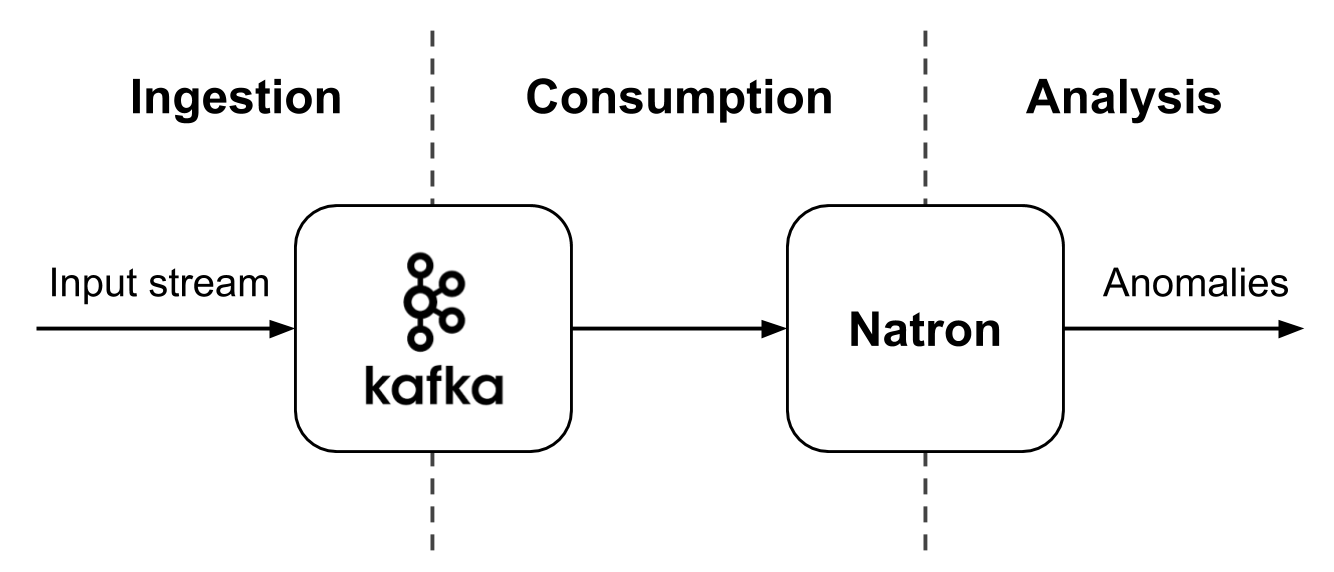
\includegraphics[width=.49\textwidth]{img/eval-arch-2}.
    }
    \subfloat[]{
      
\includegraphics[width=.49\textwidth]{img/eval-arch-3}.
    }
\caption{(a) Architecture for the single-threaded solution. (b) Architecture for the distributed solution}
\label{fig:arch_impl}
\end{figure}

In this work, we use Kafka (see Section~\ref{sec:kafka}) as our streaming data storage. We use two different configurations, one for each solution. The single-threaded solution, based on \sti{}, reads data from a single VM1 machine. The distributed solution, based on \sparkdi{}, reads data from a Kafka cluster composed of four VM2. In the distributed setting, we set the number of partitions for each topic to eight. We choose this value by considering the number of executors used in the experiments, since executors can read in parallel from different partitions.

In the single-threaded solution, the consumption phase is implemented using a Kafka Ingester that polls the data from the server in comma separated value format. The architecture for this solution is depicted in Figure \ref{fig:arch_impl}(a). The Ingester connects to an Apache Kafka server that provides the data. The data enters the system as a stream of generic objects. Each object contains its event timestamp. Downstream to the Ingester, a Processor takes the data from the Bus and transforms each element into a domain-specific Java object (i.e. a Java representation of a CDR, named PixelCDR).

Then, an Processor based on Esper (see Section~\ref{sec:esper-epl}) performs the analysis. The internal stream of PixelCDRs flows into Esper, which performs the query presented in Listing~\ref{lst:epl_query}. The query counts, every 15 minutes, the number of calls/SMSs grouped by pixelId, i.e. the pixel identifier.
The window operation is performed on the event timestamp. We use Kafka exactly-once message delivery to analyze the whole data stream. The query produces the list of anomalous pixels.
The anomalies are identified using the \textit{isAnomalous} user defined function, that access the models file, stored in memory, and implements Equation~\eqref{eq:zscore}.
The query results are then saved to the file system by an Emitter.

\begin{figure}[ht]
\begin{minipage}{0.95\linewidth}
\begin{lstlisting}[caption={EPL query performed by Esper Processor.},frame=single,captionpos=b,label=lst:epl_query,style=ESPER]
SELECT pixelId, MAX(timestamp)
FROM PixelCDR.WIN:EXT_TIMED_BATCH(timestamp, 15 min) 
GROUP BY pixelId 
HAVING isAnomalous(pixelId, COUNT(*), MAX(timestamp))
\end{lstlisting}
\end{minipage}
\end{figure}

We implemented our distributed streaming pipeline using \sparkdi{} and we register both the static models table, and the CDR data stream as temporary views that can be queried through the Structured Streaming API. The CDR view is actually a dynamic table that gets updated as data is ingested. The anomaly detection method is implemented as a SQL query that performs a join on the aforementioned tables, and filters the results based on the anomaly condition defined in Equation \eqref{eq:zscore}. Listing \ref{lst:sql_query} contains the pseudocode for the query.

\begin{figure}[ht]
\begin{minipage}{0.95\linewidth}
\begin{lstlisting}[caption={Spark SQL anomaly detection query.},frame=single,captionpos=b,label=lst:sql_query,style=SPARKSQL]
SELECT pixelId, timestamp
FROM (
	SELECT cdrs.pixelId, cdrs.timestamp, COUNT(1)
	FROM cdr_stream AS cdrs
	WINDOW ON cdrs.timestamp EVERY 15 minutes
	GROUP BY cdrs.pixelId
) AS windowed_cdrs LEFT JOIN models 
ON models.timestamp = windowed_cdrs.window.start 
WHERE isAnomalous(windowed_cdrs.value, model.mean, model.sd)
\end{lstlisting}
\end{minipage}
\end{figure}

The distributed application is deployed on a multi-node Spark cluster, while data is ingested from a multi-node Kafka cluster. This deployment is represented in Figure \ref{fig:arch_impl}(b). Spark is integrated with Kafka to provide parallel reads from multiple Kafka partitions. 

We choose Apache Spark for our distributed solution due to its wide spread use in industry, and the availability of previously developed source code and expertise.
%%
%\subsubsection{Operational considerations}
Operational requirements are related to business choices (see Section~\ref{sec:uda-analysis}). They deal, for example, with how often a result report should be produced. We consider the following two operational scenarios:
\begin{itemize}
\item \textit{Continuous ingestion -- continuous consumption and analysis}. This scenario includes real-time use cases, such as crowd monitoring for security purposes. Data is consumed as soon as it is produced, and the delay with which results are produced corresponds to the latency of the system. In this regime, results are produced continuously with whatever latency the system might have. This scenario requires the continuous utilization of reserved resources, since the solution must run without interruptions.
\item \textit{Continuous ingestion -- periodic consumption and analysis}. Periodic analysis represents a common scenario. In many use cases, the results of the analysis can be summarized in a periodic report, and the real-time analysis is not necessary. The ingestion layer must still run continuously to avoid data losses. On the other hand, the analysis layer can be allocated only for the amount of time needed to perform the analysis and generate the results.
\end{itemize}

Another important considerations when designing an industrial analytics system are fault-tolerance and redundancy. Apache Kafka and Apache Spark respectively provide out-of-the-box redundancy and fault-tolerance. Nonetheless, we do not include these aspects in our analysis, since the total solution cost of a fault-tolerant system can be approximated as the total solution cost multiplied by the redundancy factor. If we apply this consideration to both solutions, it does not affect our final results.

\subsection{Experimental Settings}
The goal of our experimental methodology is to find the most cost-effective solution for the given problem. To assess this, we run our solutions on both real and simulated problem instances. The real data MOB1 is collected from the mobile phone network of TIM. Starting from this real data we generated several other datasets (MOB10, MOB30, etc.). Those datasets were generated to analyze the scalability of our solutions. 

We compare our solutions based on their total cost when they both provide correct results. This is not always the case since the most economic single-threaded configurations struggle to deal with the most demanding problem instances. The solution cost is computed by multiplying the cost of the solution (i.e., price-per-second of the used VMs) with the execution time of the experiment (if completed correctly). The cost of the solution also depends on the operational requirements, e.g., a continuous solution can run on reserved instances, thus reducing the price-per-second.

We executed all experiments on Microsoft Azure Linux VMs. For each experiment, we performed five experimental runs. All reported results are average over four runs by discarding the worst outcome. We do not include error bars in the plots since their bounds are so tight that they simply overlap with the point shapes and clutter the images.

We do not consider latency in our analysis due to the following reasons:
\begin{enumerate}
\item In the continuous analysis scenario, at regime the latency of the system does not influence the stream of results. Moreover, the latency to analyze one minute of data is below 1.5 seconds for both solutions, which is appropriate for our use case.
\item In the periodic analysis scenario, the latency of both systems is negligible with respect to the periods considered (i.e. every day or every week).
\end{enumerate}
Thus, in the following we omit latency from our discussion.

%\subsubsection{Configurations}
Our goal is to find the most cost-effective configuration which solves the problem. We restrict our analysis to Fsv2-series VMs under the assumption that in cost-aware scenarios more general-purpose VMs are preferable to workload-optimized VMs, since they can be shared and used by different workloads. Figures \ref{fig:tuning}(a) and \ref{fig:tuning}(b) show the solution cost as a function of the scale factor for different configurations of \sti{} and \sparkdi{}. 

%\paragraph{\sti{} deployment}
\sti{} was deployed using a docker container to create a sandbox environment and to ease the monitoring operations for CPU and memory consumption. The whole infrastructure needed a single VM for each experiment in addition to the VM needed for the data provider,  i.e. a single partition Kafka server on a VM1.
We run multiple experiments for each dataset and remove the outliers, e.g. the first run of each experiments was considered as a system setup, collect data result for correctness check, i.e. anomalies, and CPU/memory consumption log to monitor the health of the infrastructure. During each run the container exploits all available virtual machine resources for the computation. We vary the dimension of the VMs in azure to stress the environment and get the upper limit of the resource needed to handle a given amount of data.

We experimented with three configurations, having different number of cores, RAM, disk I/O, and network I/O available: (i) \sti{}1 with a single VM1, (ii) \sti{}2 with a single VM2, and (iii) \sti{}3 with one VM4.

The single-threaded implementation suffers from the volume of the data, a single VM cannot scale horizontally to deal with a continuously increasing amount of data. 
Figure~\ref{fig:tuning}(a) clearly shows that the different configurations can bear different loads of data.
\sti{}1 can handle dataset MOB1, which represents the original data size, and can perform the anomaly detection in about 120 seconds. This configuration can handle up to dataset MOB10, but bigger dataset results are problematic. Configurations \sti{}2 and \sti{}3 can bear at most dataset MOB50 and MOB100  (respectively), but are more expensive than configuration \sti{}1 .
The three chosen configurations widely explore the hardware offerings in order to find the best solution related to the data loads. Due to the variability of configurations' behaviors, we tested the system against more dataset than the ones listed in Section~\ref{sec:desc}, i.e. we tested dataset with scale factor k=2, k=3, k=5, and k=20.

We compare all the three \sti{} configurations with the best configuration chosen for the distributed system in order to have a complete overview for the different input volumes. During the experiments, regardless of the \sti{} configuration, the normality models are loaded in memory, while streaming data is read from the Kafka cluster described in Section \ref{sec:kafka}.

%%
%\subsubsection{\sparkdi{} deployment}
We deployed \sparkdi{} application on a Spark cluster tuned using the total solution cost as a metric, and experimenting with three parameters which commonly affect Spark's performance. Our intention here is to present our findings on the best Spark configuration for our specific use case, datasets, and problem setting. We implemented our Apache Spark cluster using Azure Linux VMs (see Table \ref{tab:sizes}).

\begin{figure}[t!]
  \subfloat[]{
    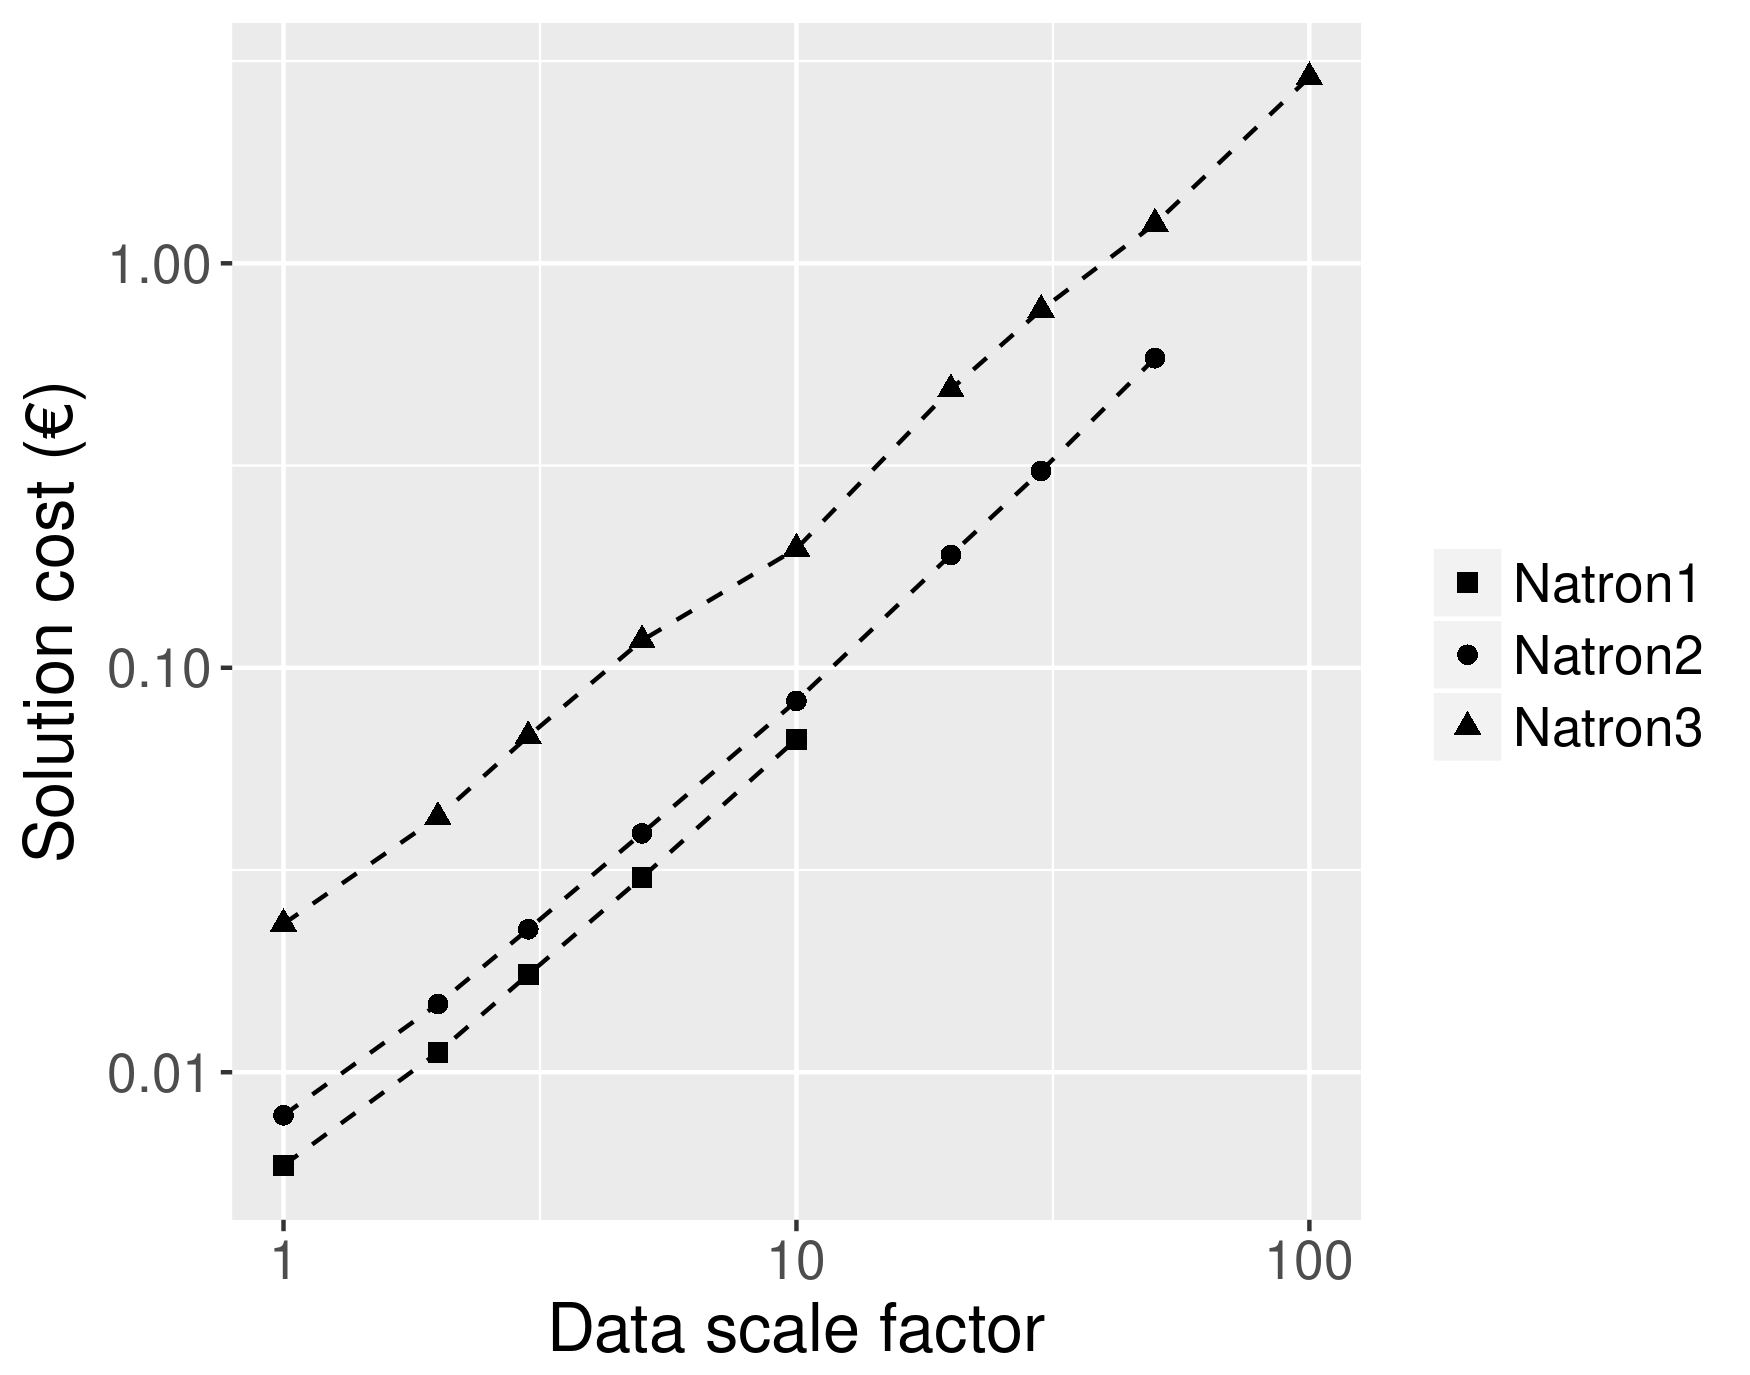
\includegraphics[width=.49\textwidth]{img/eval-natron_base}.
  }
  \subfloat[]{
    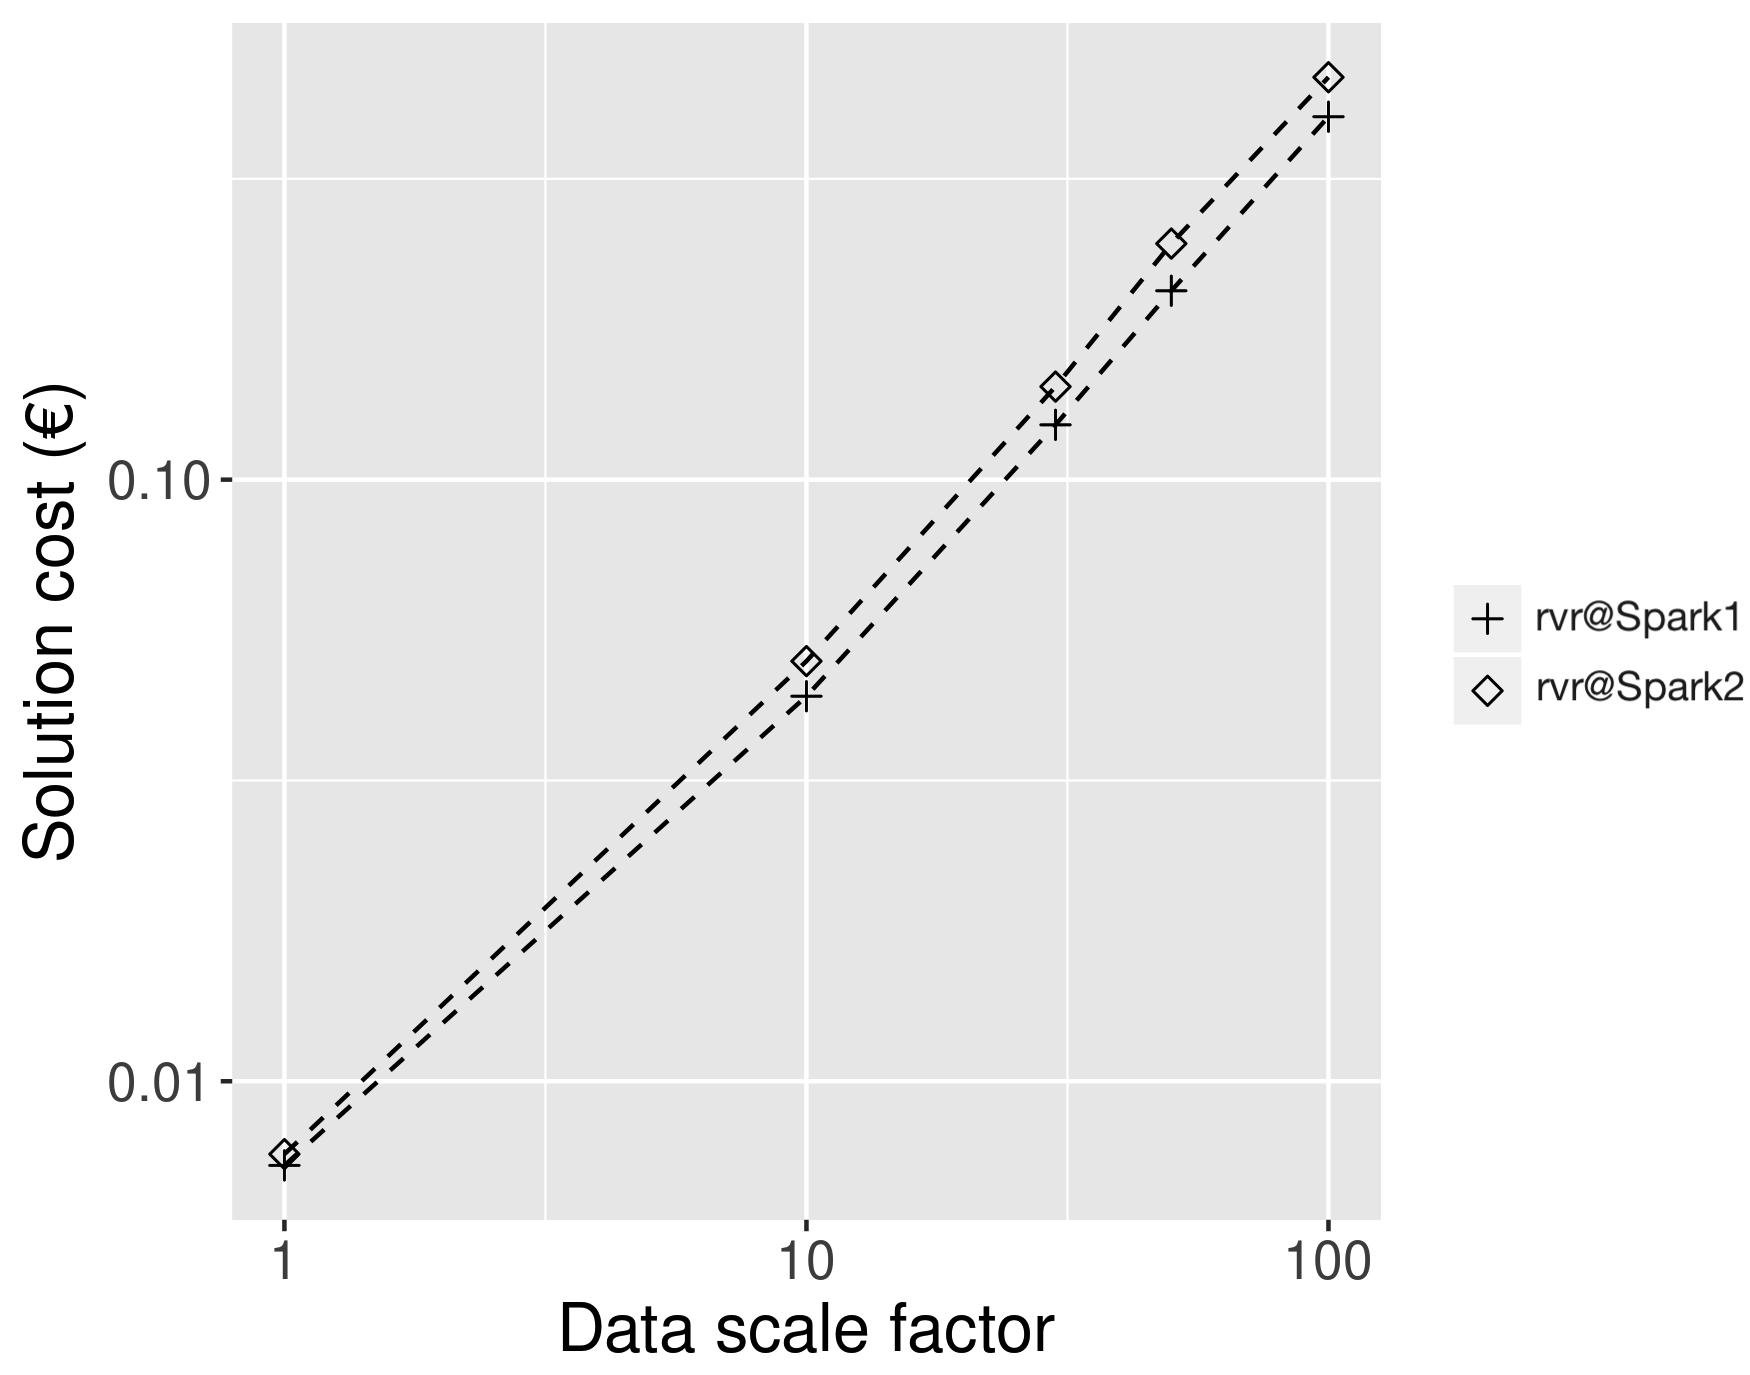
\includegraphics[width=.49\textwidth]{img/eval-spark_time_vs_size}.
  } \\
  \subfloat[]{
    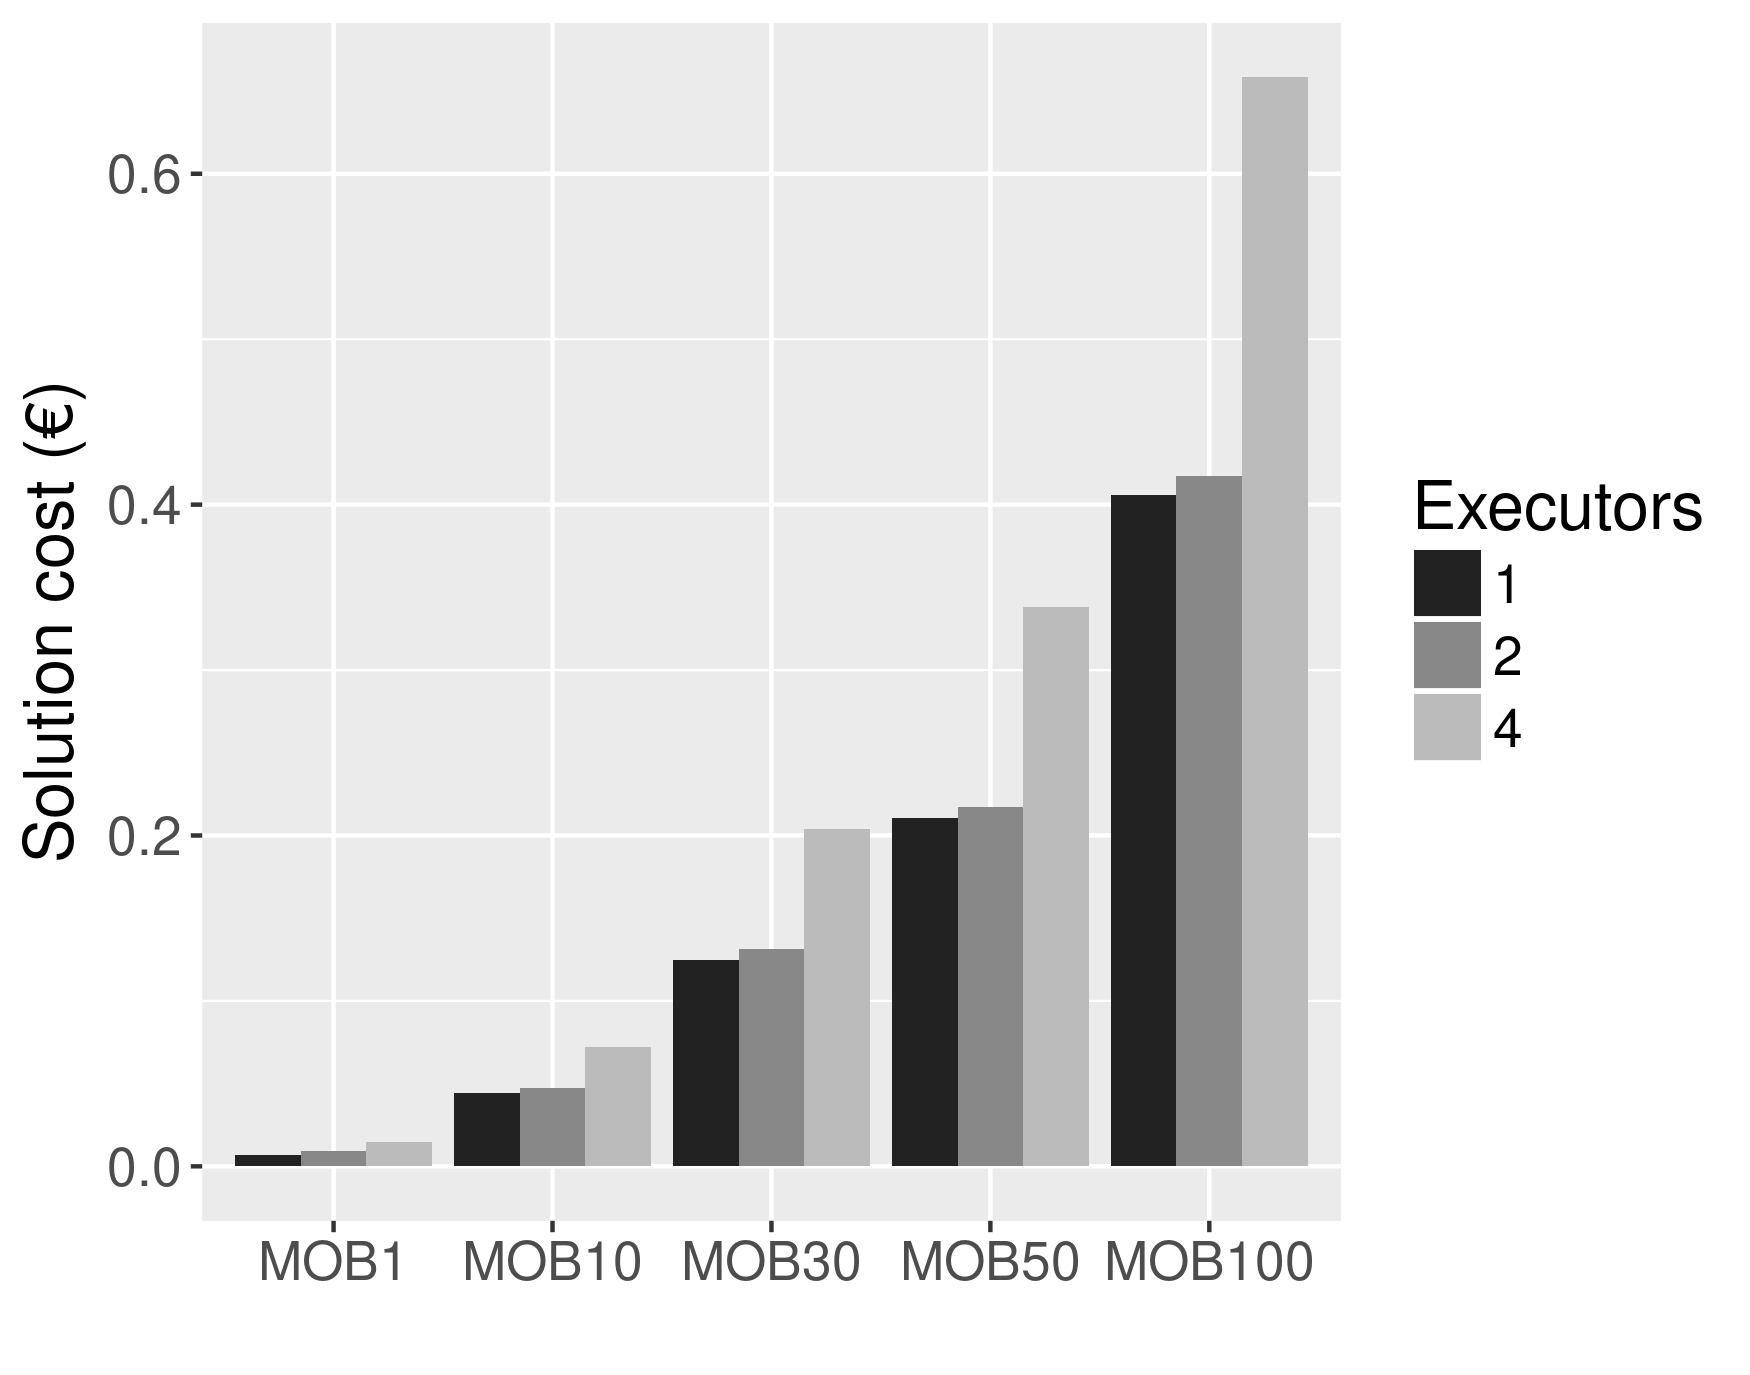
\includegraphics[width=.49\textwidth]{img/eval-spark_time_vs_executors}.
  }
  \subfloat[]{
    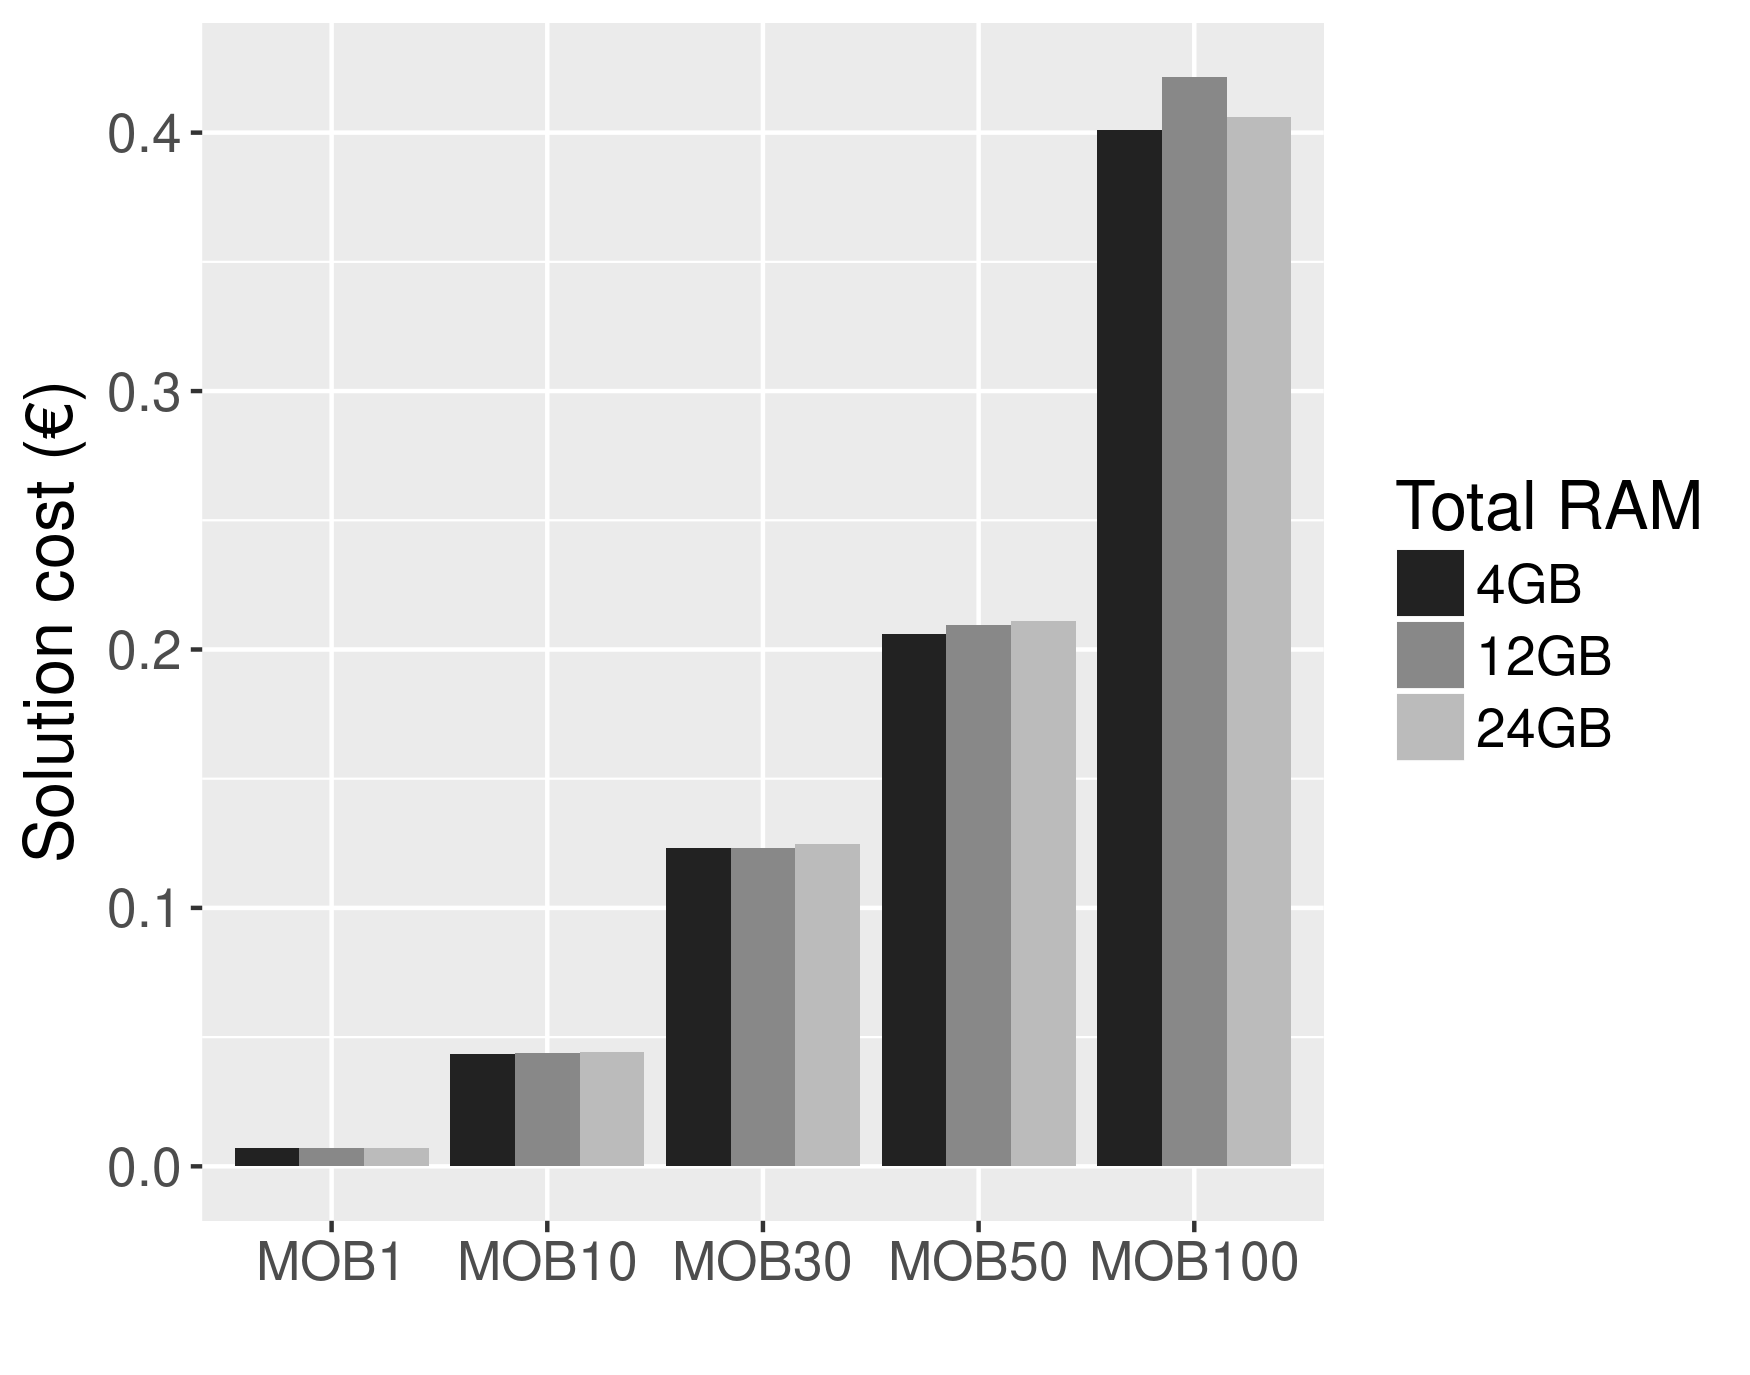
\includegraphics[width=.49\textwidth]{img/eval-spark_time_vs_ram}.
  }
\caption{(a) Solution cost over data scale for different \sti{} configurations. (b) Solution cost over data scale for different \sparkdi{} configurations. (c) Solution cost over number of executors per worker on different datasets (RAM at 24GB). (d) Solution cost over total number of RAM in GB for different datasets (1 executor per worker).}
\label{fig:tuning}
\end{figure}

We experimented with the following cluster parameters: i)the virtual machine size, ii) the number of executors per worker (or number of cores per executor), and iii) the memory allocated per executor.
All other parameters were set to their default values. Note that, since in Microsoft Azure each virtual core (vCPU) corresponds to a single thread, in the following we use the terms core and thread interchangeably.
%%

%\subsubsection{Virtual machine size} 
Cloud service providers offer several VM types. Those types vary depending on the number of cores, RAM, disk I/O, and network I/O available to user applications running on the VM. Thus, an important consideration when deploying a cloud solution is the choice of VM type.

We evaluated two different cost-equivalent configurations for our Spark cluster (refer to Table \ref{tab:sizes} for VM characteristics): (i) \sparkdi{}1 with one VM2 as a master and four VM2 workers, and (ii) \sparkdi{}2 with a singly VM2 as a master and two VM3 workers.

Note that we also experimented with smaller cluster configurations (e.g., a single VM2 worker). However, we found that these were not as cost-effective as the configurations described above. This might seem counterintuitive. However, consider that a smaller configuration usually takes more time to perform the analysis. Since our metric is the total solution cost, to be cost-effective a solution's cost reduction should compensate for its performance penalty.

As an example, we found out that a cluster with a single VM2 worker takes from 2.75 to 3 more time (depending on the dataset) to perform the task with respect to our \sparkdi{}1 configuration, while only costing 2.5 less.

Figure \ref{fig:tuning}(b) shows the cost of the solution for both configurations. All Spark settings were set to their default values (all available cores, 1GB of RAM per executor). The figure highlights that the \sparkdi{}1 configuration tend to be more cost-efficient, even though the total number of used cores is the same in both configurations.

Even after tuning both clusters, i.e. by changing the default parameters, we could not find a configuration for \sparkdi{}2 outperforming \sparkdi{}1. We used \sparkdi{}1 for all other experiments. The two following sections provide more details on the experiments we performed measuring the sensitivity of the selected configuration to changes in the number of cores per executor and in the amount of RAM per executor.

%\subsubsection{Cores per executor} 
An important parameter in Spark configuration is the number of cores allocated to each executor. The default configuration allocates all available cores. Incidentally, the number of cores per executor also determines the number of executor processes that a worker can spawn. Thus, we perform our sensitivity analysis in term of executors per worker. We fixed the total RAM to 24GB and varied the number of executors per worker machine. Figure \ref{fig:tuning}(c) shows our results. We can see that having a single executor on each worker outperforms other configurations. This is supposedly due to the fact that when multiple executors reside on the same machine, the JVM must handle a large volume of I/O network traffic in order for them to communicate. This could possibly influence application performance.

%\subsubsection{RAM per executor} 
Another important parameter is the amount of RAM designated to each executor. In this case, we picked the best configuration from the previous analysis, i.e. one executor per worker, and varied the RAM allocated to each executor. Figure \ref{fig:tuning}(d) shows our results to this sensitivity analysis. We can notice that the amount of memory allocated to each executor does not seem to affect execution time. This is surprising, considering the common knowledge that Spark performance is proportional to the amount of main memory available. However, our particular use case, i.e. windowed and watermarked relational query, is executed considering one window of data at a time. Even at maximum scale (x100), our windows do not exceed 1GB of RAM, and therefore in this particular scenario the system is not memory-bounded.

All the following experiments were executed using configuration \sparkdi{}1 with 4 cores and 3GB of RAM per executor. The normality models are stored in a static file over the Spark cluster, while streaming data is read from the Kafka cluster described in Section~\ref{sec:kafka}.

\subsection{Results and Discussion} \label{sec:results}

\begin{table}[ht]
\centering
\caption{Operational scenarios. Each layer of the system can run continuously (C) or periodically (P), and on shared (S) or reserved (R) hardware. Data ingestion and consumption are both handled by Apache Kafka, therefore they are always executed on the same hardware.}
\begin{tabular}{@{}lrrr@{}} \toprule
Scenario & Ingestion & Consumption & Analysis \\
\midrule
S1 & C/R & C/R & C/R \\
S2 & C/R & P/R & P/S \\
\bottomrule
\end{tabular}
\label{tab:scenarios}
\end{table}

In this section, we present our experimental results. We organize our discussion based on the operational requirements considered in Section \ref{sec:solutions}. The analyzed scenarios are summarized in Table \ref{tab:scenarios}. 

\begin{table}[ht]
\centering
\caption{Monthly solution costs. The monthly cost of our solution depending on the operational scenario. Notice that if we perform continuous ingestion, the consumption costs are included (Incl.). The third scenario represents the case in which ingestion costs are fixed, i.e. they do not depend on the number of machines, but only on data throughput. The most cost-effective solution is highlighted.}
\begin{tabular}{@{}llrrrr@{}} \toprule
Scenario & & Ingestion & Consum. & Analysis & Total\\
\midrule
S1 & \sparkdi{}1 & \euro486.32 & Incl. & \euro607.9 & \euro1094.22 \\
   & \sti{}3 & \euro60.33 & Incl. & \euro484.92 & \textbf{\euro545.25}\\
\midrule
S2 & \sparkdi{}1 & \euro486.32 & Incl. & \euro12,41 & \euro498,73\\
   & \sti{}3 & \euro60.33 & Incl. & \euro76.85 & \textbf{\euro137.18}\\
\midrule
S3 & \sparkdi{}1 & Fixed & \euro9.93 & \euro12.41 & \textbf{\euro22.34}\\
   & \sti{}3 & Fixed & \euro9.68 & \euro76.85 & \euro86.53\\
\bottomrule
\end{tabular}
\label{tab:monthly}
\end{table}

The resulting monthly solution costs per scenario are represented in Table \ref{tab:monthly}. All costs refer to the MOB100 dataset. Periodic scenarios (S2 and S3) refer to analysis carried out daily, i.e., 30 times per month.

\begin{figure}[p]
  \centering
  \subfloat[]{
      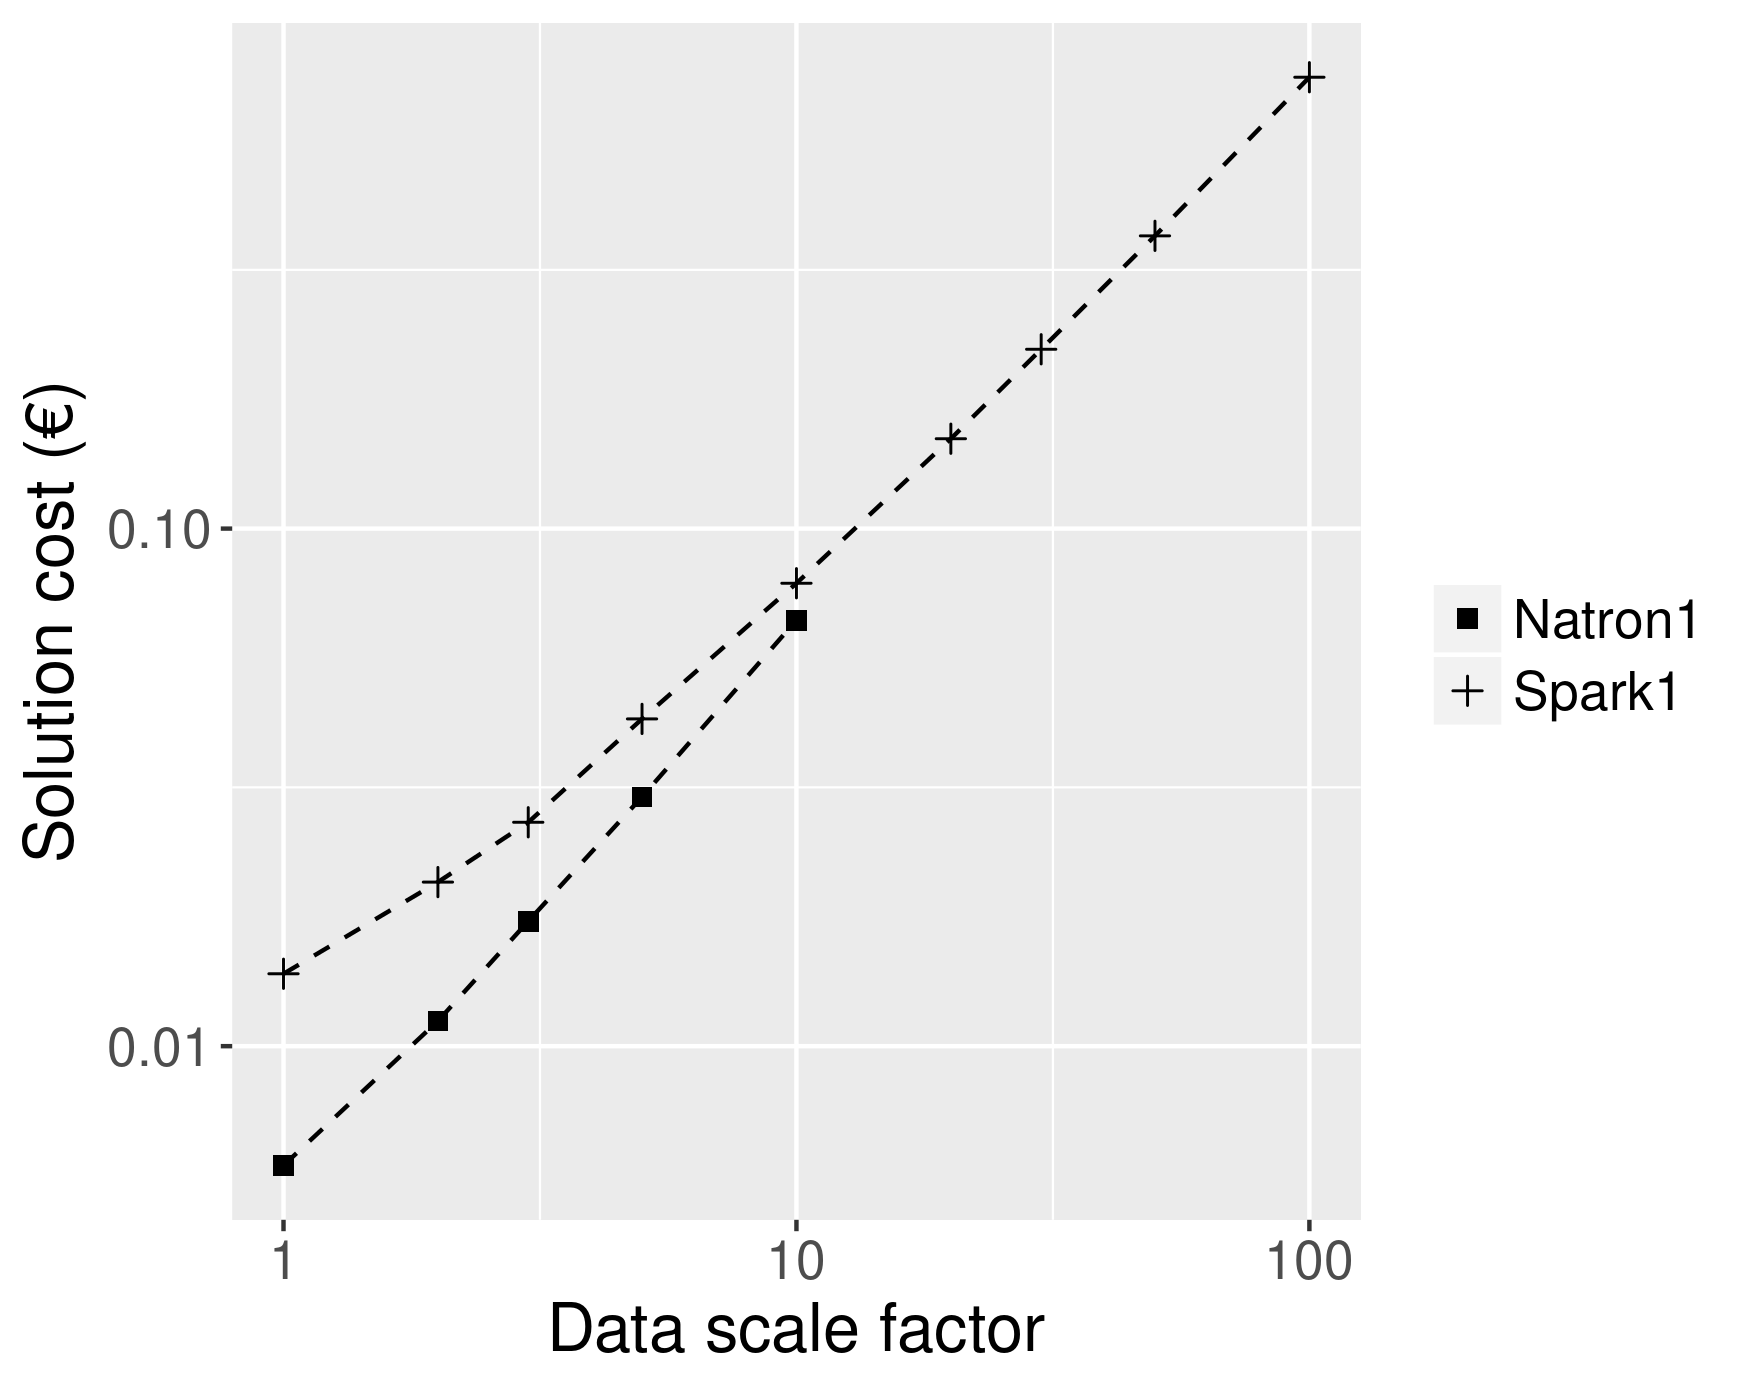
\includegraphics[width=0.47\textwidth]{img/eval-N1_vs_spark}.
    } 
    \subfloat[]{
      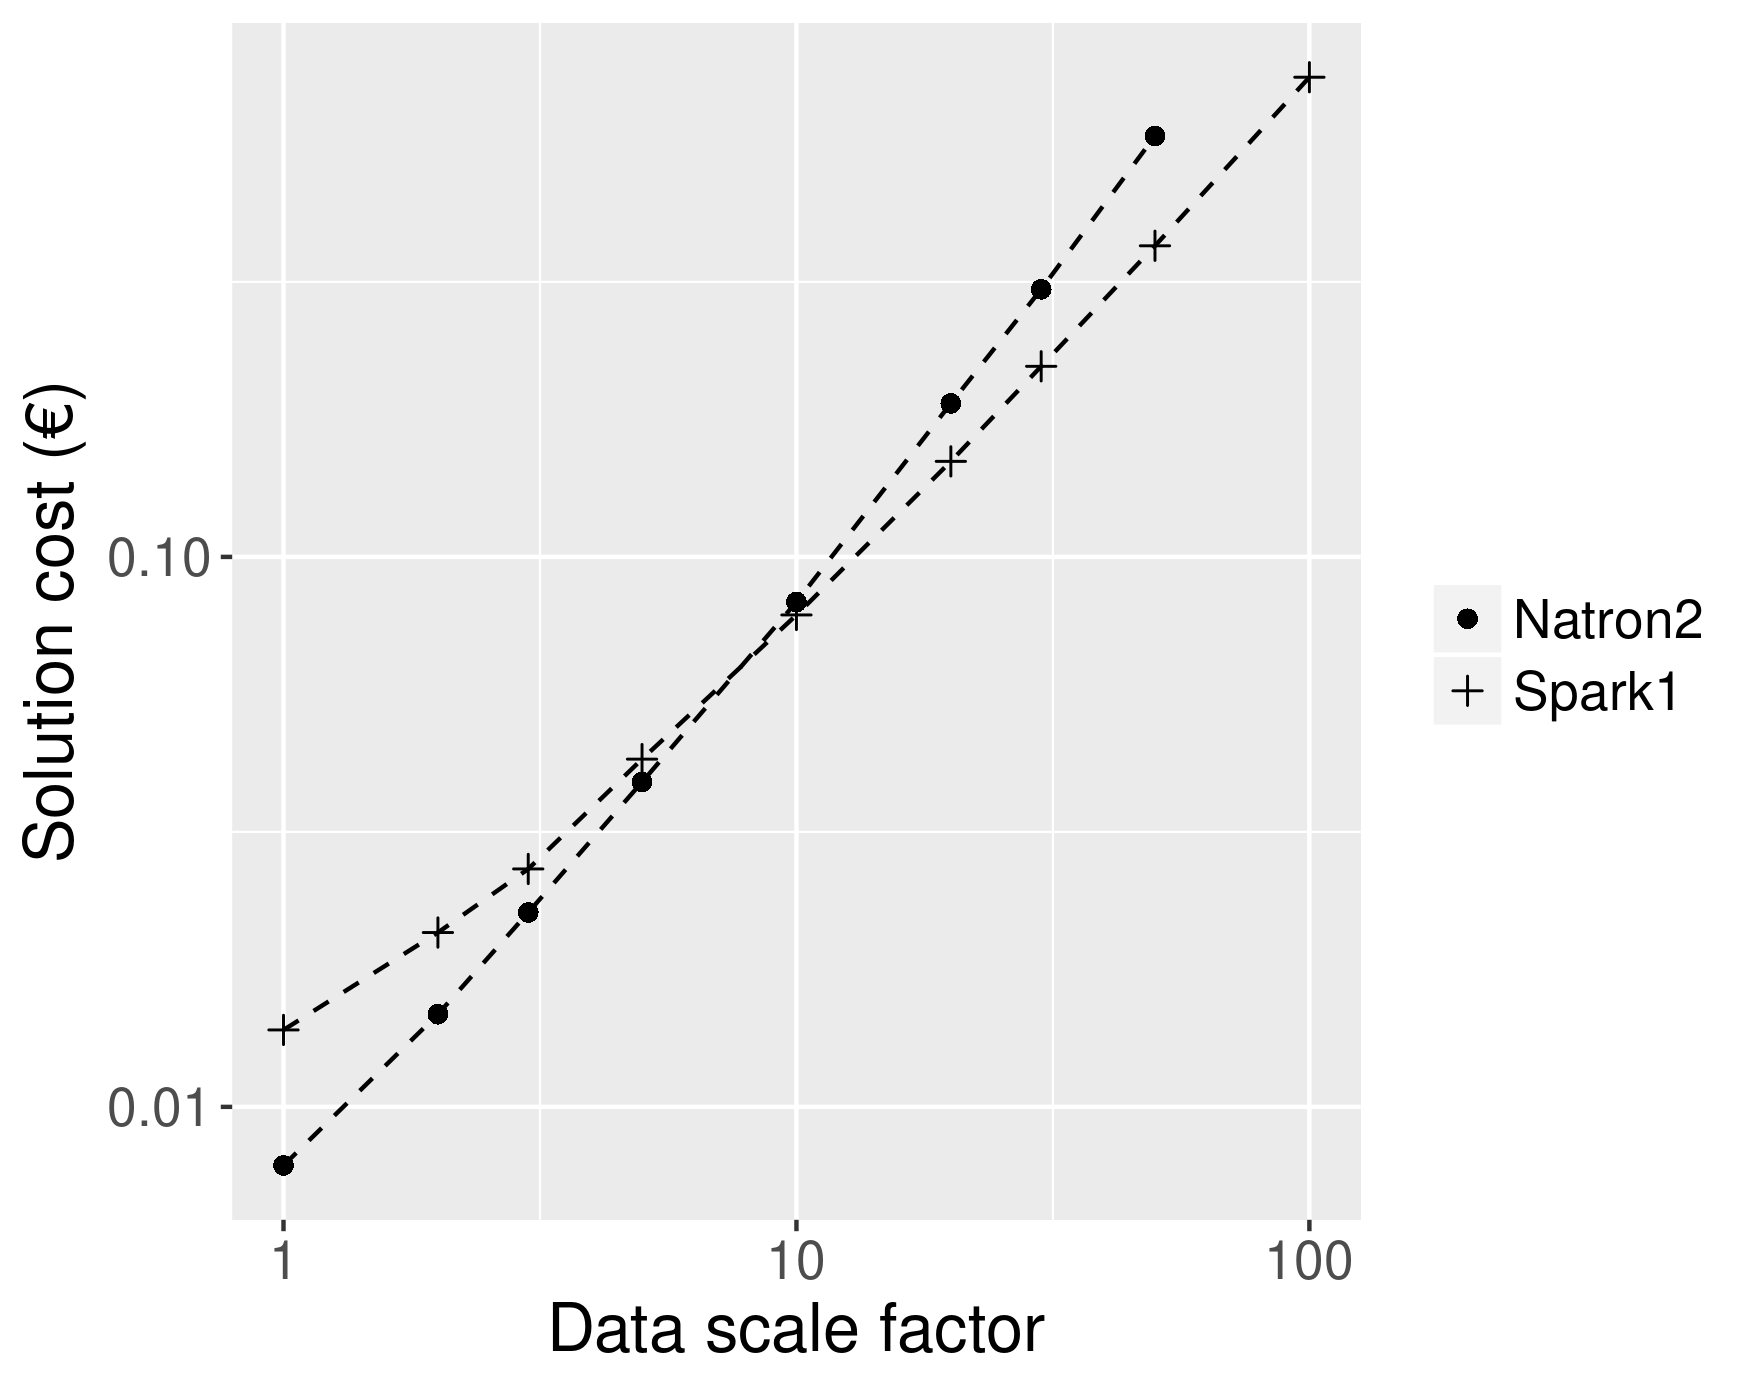
\includegraphics[width=0.47\textwidth]{img/eval-N2_vs_spark}.
    }\\
    \subfloat[]{
      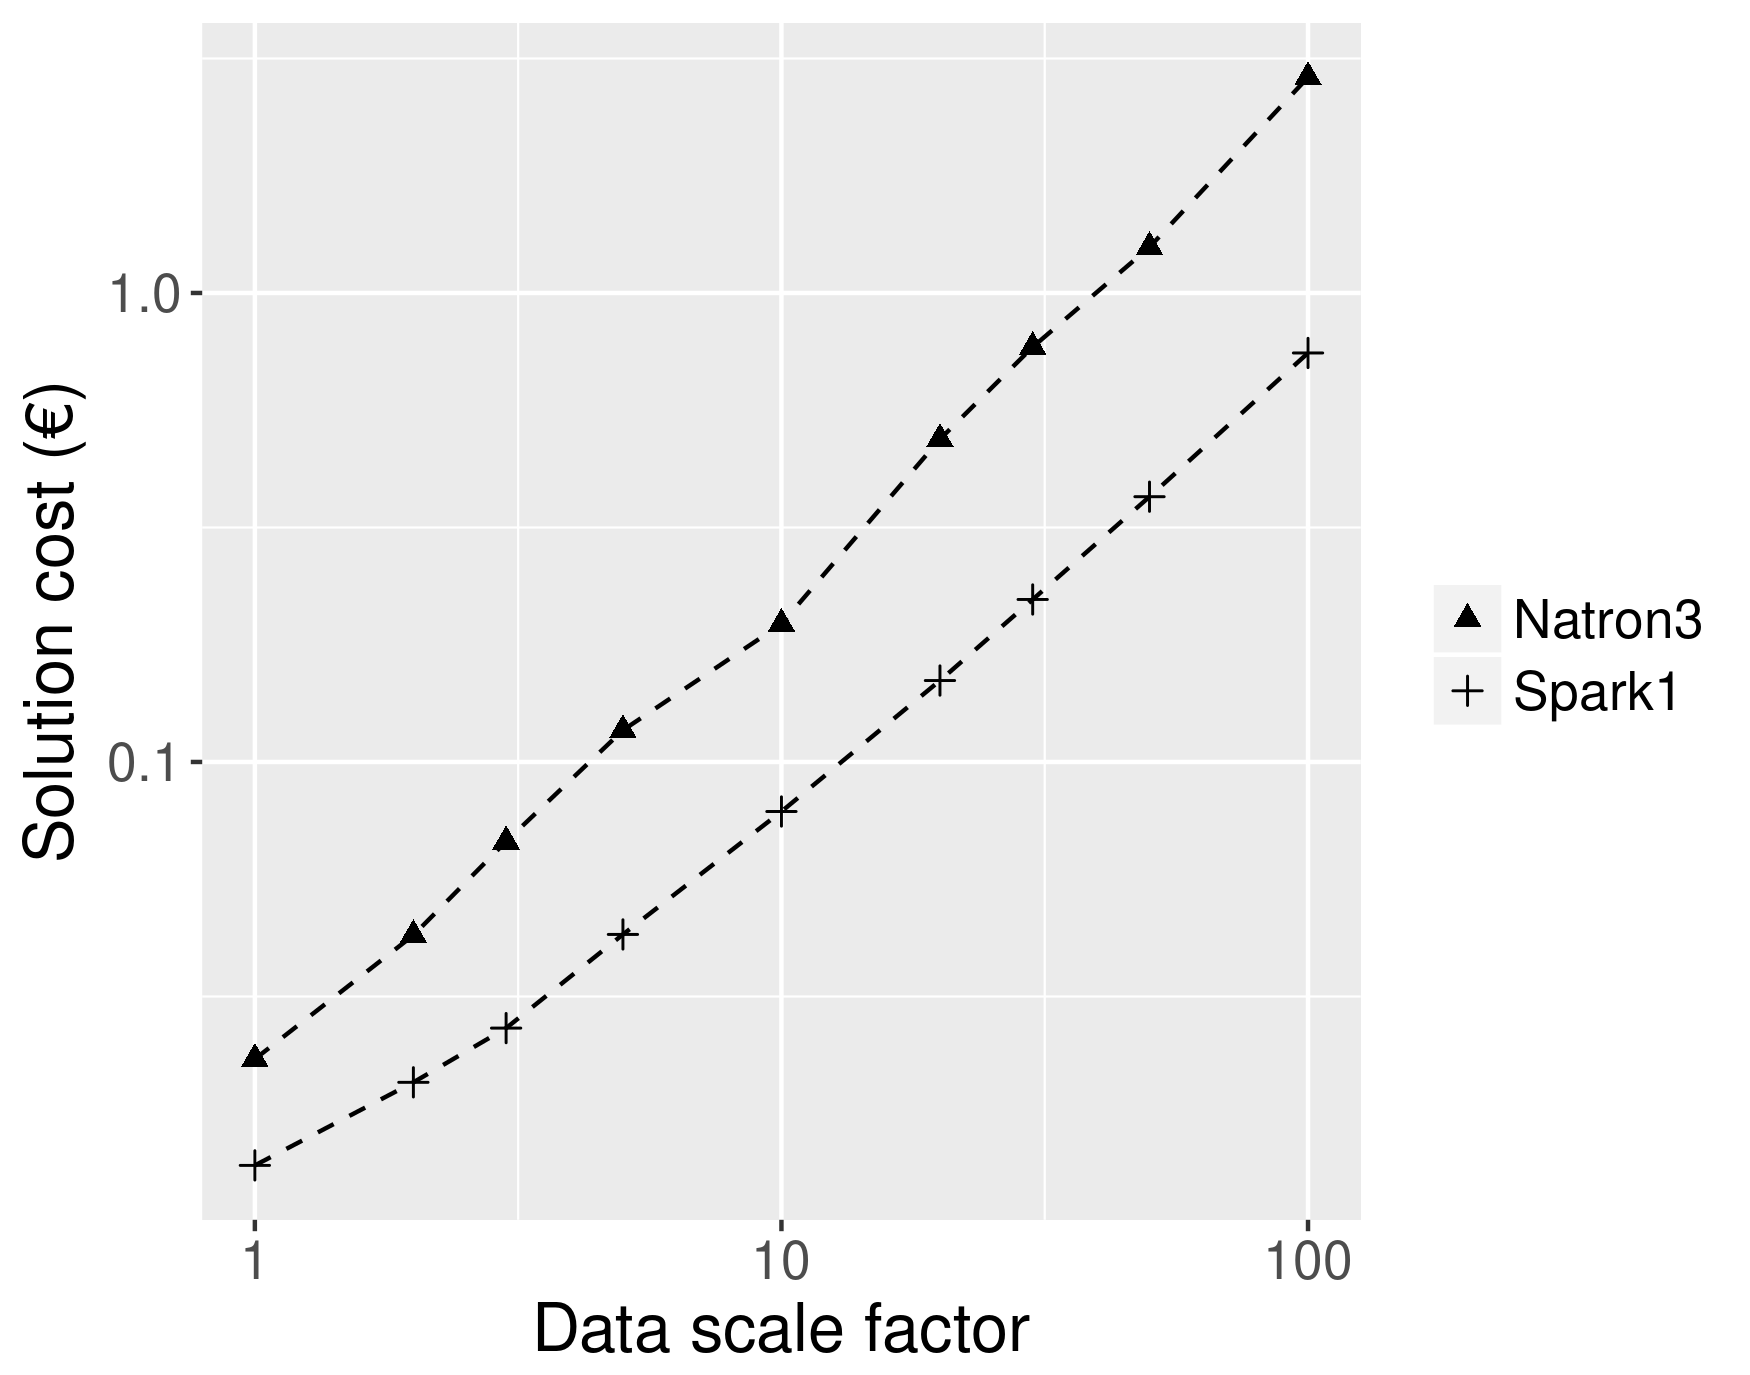
\includegraphics[width=0.47\textwidth]{img/eval-N3_vs_spark}.
    }
\caption{(a) Total solution cost for S3: \sti{}1 vs \sparkdi{}1. \sti{}1 is the lowest cost solution, but it can handle only datasets of modest size. (b) Total solution cost for S3: \sti{}2 vs \sparkdi{}1. The two solutions are cost-equivalent at a scale factor around 10. After that, \sparkdi{}1 becomes the most cost-effective solution. (c) Total solution cost for S3: \sti{}3 vs \sparkdi{}1. \sti{}3 can handle all datasets considered, however it is less cost-effective than the distributed system at all scales.}
\label{fig:NvsSpark}
\end{figure}

\medskip

\textit{S1 -- Continuous ingestion -- continuous consumption and analysis}
In this scenario, we consider the case in which we require a continuous analytics solution. The whole infrastructure must be continuously up and running to support the ingestion, consumption and analysis phases. We can compute a monthly solution cost by considering the reservation price of all VMs used in the solution. 

From Table \ref{tab:monthly}, we can see the estimated monthly solution cost for scenario S1. Ingestion cost is calculated using reserved instance price, since these machines must run continuously. This is the same for analysis cost. Consumption cost is included in the ingestion, since the Kafka VMs perform both phases continuously. The single-thread cost is calculated considering configuration \sti{}3. 

In this case, we can clearly see that the single-threaded implementation is the most cost-effective solution for the problem.

\medskip

\textit{S2 -- Continuous ingestion -- periodic consumption and analysis}
This scenario represents a use case where the continuous analysis is not necessary, but periodic reports are needed. Table \ref{tab:monthly} contains the cost analysis for this scenario. The costs of ingestion and consumption are equivalent to S1. The analysis cost is computed on the more demanding dataset MOB100, using \sparkdi{}1 and \sti{}3 configurations. We report the monthly cost for an analysis performed daily. The ingestion phase must be continuous and, consequently, the infrastructure that support the ingestion and consumption phases can be deployed on reserved hardware. The analysis is periodic (once a day), and can be executed on pay-per-use VMs which can be turned on only for the duration of the analysis. 

In this scenario, we can see that the \sparkdi{} system is more cost-effective with respect to the analysis phase, but not to the ingestion phase. The cost of continuously ingesting data using a distributed cluster outvalues the benefits of processing such data in parallel. This is still true at lower data scales, where the convenience of the single-threaded solution is even more evident.

After realizing this fact we included a final scenario (\textit{S3}) in our analysis. This scenario is a situation where data ingestion is provided at a fixed and small price, i.e. it does not depend on VMs cost but only on data throughput and retention. This is the case with some particular offers from cloud providers such as Confluent\footnote{\url{https://www.confluent.io}}. Since the throughput and the retention are fixed, in this scenario the ingestion cost is the same for both solutions.

\medskip

\textit{S3 -- Continuous ingestion at fixed/small price -- periodic consumption and analysis}
In this scenario the total cost of the solution depends on the number of machines active during the analysis phase, and on the duration of this phase. Thus, if the additional costs of using more machines in the distributed setting implies reducing the execution time by the same factor, then the distributed solution is the most cost-effective.

Table \ref{tab:monthly} presents the results for this scenario. The results  compare configuration \sparkdi{}1 versus configuration \sti{}3 when processing the dataset MOB100. We assume the analysis is carried out periodically each day. We can see that the reduced execution time for the analysis makes up for the increased number of VMs. This makes the distributed solution around 3.8 times more cost-efficient than the single-threaded system.

We provide more insight on this scenario by considering different data scales. We compare configuration \sparkdi{}1 with the less expensive \sti{} configuration that can handle a given data scale: configuration \sti{}1 for a scale factor up to 10, configuration \sti{}2 for a scale factor up to 50, and configuration \sti{}3 for the dataset MOB100.

We can see that, in this setting, the most cost-effective solution depends on the data size. At small data scales, configuration \sti{}1 is the most cost-effective solution. The configuration \sti{}1  can only deal with data volumes up to scale factor 10 (city scale), but, until this point, it is more cost-effective than configuration \sparkdi{}1 (Figure~\ref{fig:NvsSpark}(a)). When the data size increases, the solutions first become equivalent in term of cost around city scale (Figure~\ref{fig:NvsSpark}(b)), and, then, configuration \sparkdi{}1 becomes the most cost-effective solution (Figure~\ref{fig:NvsSpark}(c)) when dealing with national and extreme scales.

The results presented in this section show that in case of continuous analysis, the single-threaded solution is the most cost-effective option.

When periodic analysis is considered, the distributed solution is the most cost-effective in analyzing the data. However, this benefit is outvalued by the costs of distributed data ingestion. Thus, the single-threaded application remains the best choice also in this case.

Finally, if we assume that data ingestion costs only depends on data throughput and retention, i.e. they are fixed and small, we show that the most cost-effective choice depends on the data size. The single-threaded application is cost-effective when managing small datasets, which is our setting are the CDRs generated by Milan when including Internet or those of the entire Italy if limiting the analysis to calls and SMSs. However, as the data size grows to the size of Italy including Internet, the distributed solution becomes the most cost-effective option.

\section{Conclusion}

In this chapter, we investigate how to implement \river{} computational model from different points of view.
We concentrate our effort on the implementation of the \textit{Lazy Transformation} approach.

We present \sti{} (see Section~\ref{sec:comp-mod-impl-v}) -- a single-threaded, vertically scalable implementation of the \river{} computational model -- and we evaluate it against our Streaming Linked Data Framework (SLD) that applies data transformation at ingestion time (see Section~\ref{sec:comp-mod-eval-performace}).
The result of this evaluation validates Hypothesis \textsf{Hp.2.1}: \sti{} results better than SLD under both resource consumption and correctness points of view.

Comforted by the results of this performance evaluation, we assume the \textsf{Lazy Transformation} as a third principle \textbf{(P3)} of our computational model and we apply it in the horizontally scalable implementations based on distributed technologies (see Section~\ref{sec:comp-mod-impl-h-spark} and Section~\ref{sec:comp-mod-impl-h-hive}): \sparkdi{} and \hivedi{}.

In order to reaffirm the importance of the cost-effectiveness metric in the evaluation of streaming based system, we perform an empirical comparison between \sti{} and \sparkdi{} for a streaming data analysis task (see Section~\ref{sec:comp-mod-eval-cost}).
The overall results partially validates the hypothesis \textsf{Hp.2.2}. 
\sti{} results cost-effective when managing medium size datasets (up to the scale of a large city like Milan), but, as the data size grows, \sparkdi{} becomes the most cost-effective option.